\documentclass[a4paper]{article}

%% Language and font encodings
\usepackage[english]{babel}
\usepackage[utf8x]{inputenc}
\usepackage[T1]{fontenc}

%% Sets page size and margins
\usepackage[a4paper,top=3cm,bottom=2cm,left=3cm,right=3cm,marginparwidth=1.75cm]{geometry}

%% Useful packages
\usepackage{amsmath}
\usepackage{amssymb}
\usepackage{mathtools}
\DeclareMathOperator*{\argmin}{arg\,min}
\DeclarePairedDelimiter\floor{\lfloor}{\rfloor}
\usepackage{graphicx}
\usepackage{graphics}
\usepackage{subcaption}
%\usepackage[colorinlistoftodos]{todonotes}
\usepackage[colorlinks=true, allcolors=blue]{hyperref}
\usepackage{amsthm}
\newtheorem{theorem}{Theorem}
\newtheorem{lemma}[theorem]{Lemma}
\usepackage{bbm}
\setlength\parindent{0pt}
\newcommand{\RR}{\mathbb{R}}
\renewcommand{\cal}{\mathcal}
\DeclareMathOperator*{\minimize}{minimize}
\DeclareMathOperator*{\maximize}{maximize}
\setlength{\parskip}{1em}
\newcommand{\E}{\mathbb{E}}
% \makeatletter
%   \def\title@font{\Large\bfseries}
%   \let\ltx@maketitle\@maketitle
%   \def\@maketitle{\bgroup%
%     \let\ltx@title\@title%
%     \def\@title{\resizebox{\textwidth}{!}{%
%       \mbox{\title@font\ltx@title}%
%     }}%
%     \ltx@maketitle%
%   \egroup}
% \makeatother



\title{Adaptive Piecewise Polynomial Estimation via Trend Filtering}
\author{Yandi Shen}


\bibliographystyle{plain}

\begin{document}
\maketitle
% \begin{abstract}
% Your abstract.
% \end{abstract}

% \section{Introduction Structure}
% \begin{itemize}
% \item Introduce the function estimation data model
% \item Start introducing the class of linear smoothers, and focus on smoothing splines, demonstrate that linear smoothers don't perform well for inhomogeneous function
% \item Show that theoretically, linear smoothers are suboptimal for total variation class
% \item Move onto nonlinear smoothers, three ones, show why the other two are bad
% \item introduce trend filtering
% \item briefly talk about how to extend univariate function estimation to higher dimensions
% \item briefly talk about the development of trend filtering after this paper
% \item Organizations of the rest of the paper
% \end{itemize}

\section{Introduction}
\label{sec:intro}
In this paper, we focus on univariate function estimation. We assume the following general data model:

\begin{align}
y_i = f_0(x_i) + \epsilon_i, \qquad i = 1, 2, \ldots, n  \label{nonpara_model}
\end{align}
where $\{x_1, x_2, \ldots, x_n\}\in\RR$ are one-dimensional input variable, $\{\epsilon_1, \epsilon_2, \ldots, \epsilon_n\}$ are i.i.d. errors with $E(\epsilon_i) = 0$ and $\mbox{Var}(\epsilon_i) = \sigma^2$, $\{y_1, y_2, \ldots, y_n\}$ are the observed response, and $f_0(\cdot)$ is the true regression function to be estimated. Moreover, we consider the random design setup, i.e. both input variable $x$ and noise $\epsilon$ are random variables, and we assume they are independent. 

One popular class of methods to estimate $f_0$ is the linear smoother. Many well-known estimators in literatures belong in this category: regression splines\cite{de1978practical}, kernel smoothers[Chapter 6 of \cite{friedman2001elements}, \cite{loader2006local}], $k$ nearest neighbors, smoothing splines\cite{de1978practical,wahba1990spline,green1993nonparametric}, reproduce kernel Hilbert space (RKHS) smoother\cite{smola1998learning,wahba1990spline}, sieves\cite{shen1994convergence,wong1995probability}, etc.  For linear smoothers, the estimate at arbitrary point $x$ is a linear combination of the observations $(y_1,\ldots, y_n)$. In words, there exists a weight vector $(w_1(x), \ldots, w_n(x))$ such that at any arbitrary point $x$ the estimate has the form $\hat{f}(x) = \sum_{i=1}^n w_i(x)y_i$. Thus the vector of fitted values $\hat{\mu} = (\hat{f}(x_1), \ldots, \hat{f}(x_n))$ at input points $(x_1, \ldots, x_n)$ has the matrix form $\hat{\mu}$ = $S_\lambda$y, where $S_\lambda$ is called the linear smoother matrix. The subscript $\lambda$ marks the general notion of smoothing parameter, this can be the number $k$ of chosen neighbors in $k$ nearest neighbor or the tuning parameter $\lambda$ in smoothing splines, etc. Linear smoothers have many nice properties which make them extremely useful in practice. For example, linear smoothers have closed-form degrees of freedom\cite{efron1986biased}---the trace of the smoother matrix $S_\lambda$, which facilitates model comparison. Moreover, the simple linear model leads to closed-form leave-one-out cross validation error, which makes it very efficient to choose smoothing parameter through cross validation/generalized cross validation. See Section 5.2 and 5.3 of \cite{wasserman2007all} for a more detailed discussion of linear smoothers.

However, there is one distinct drawback of linear smoothers---they are not locally adaptive. In words, they cannot represent well a signal that has a spatially heterogeneous degree of smoothness. Figure \ref{fig:homo} shows two functions with homogeneous and inhomogeneous smoothness. On the left panel, the function is equally smooth over the entire range; on the right panel the function is smoother on the left end but exhibits multiple "hills" on the right end, which gives it spatially inhomogeneous smoothness. For a heterogeneous signal like the right panel in Figure \ref{fig:homo}, linear smoothers with large degrees of freedom will under-smooth the smoother part (e.g. the left end of right plot in Figure \ref{fig:homo}), while smaller degrees of freedom will on the contrary over-smooth the wiggly part of the signal (e.g. the "hills" on the right). Let us use smoothing spline as an illustration. In Figure \ref{fig:ssvslars}, we fit smoothing splines to a dataset generated from the heterogeneous function in the right panel of Figure \ref{fig:homo}. The true function and observations with noise are shown in the top left panel. In the bottom left panel, we fit smoothing splines with 19 degrees of freedom. Now the left part of the true function is fit relatively well, however the "hills" on the right end are apparently over-smoothed. When we increase the degrees of freedom to 29 to allow more flexibility, smoothing splines is able to fit the "hills" on the right end much better but now the left part becomes much more wiggly. Such phenomenon is not restricted to smoothing splines but exists for all linear smoothers, and can be partly explained by the minimax theory briefly introduced in the next paragraph and developed in more detail in later sections. To achieve local adaptivity, people have proposed to use, for example, local bandwidth parameter in kernel smoothers or local penalty parameter in smoothing spline, but it is both difficult theoretically and practically to come up with a satisfying solution.

\begin{figure}[t!]
\centering
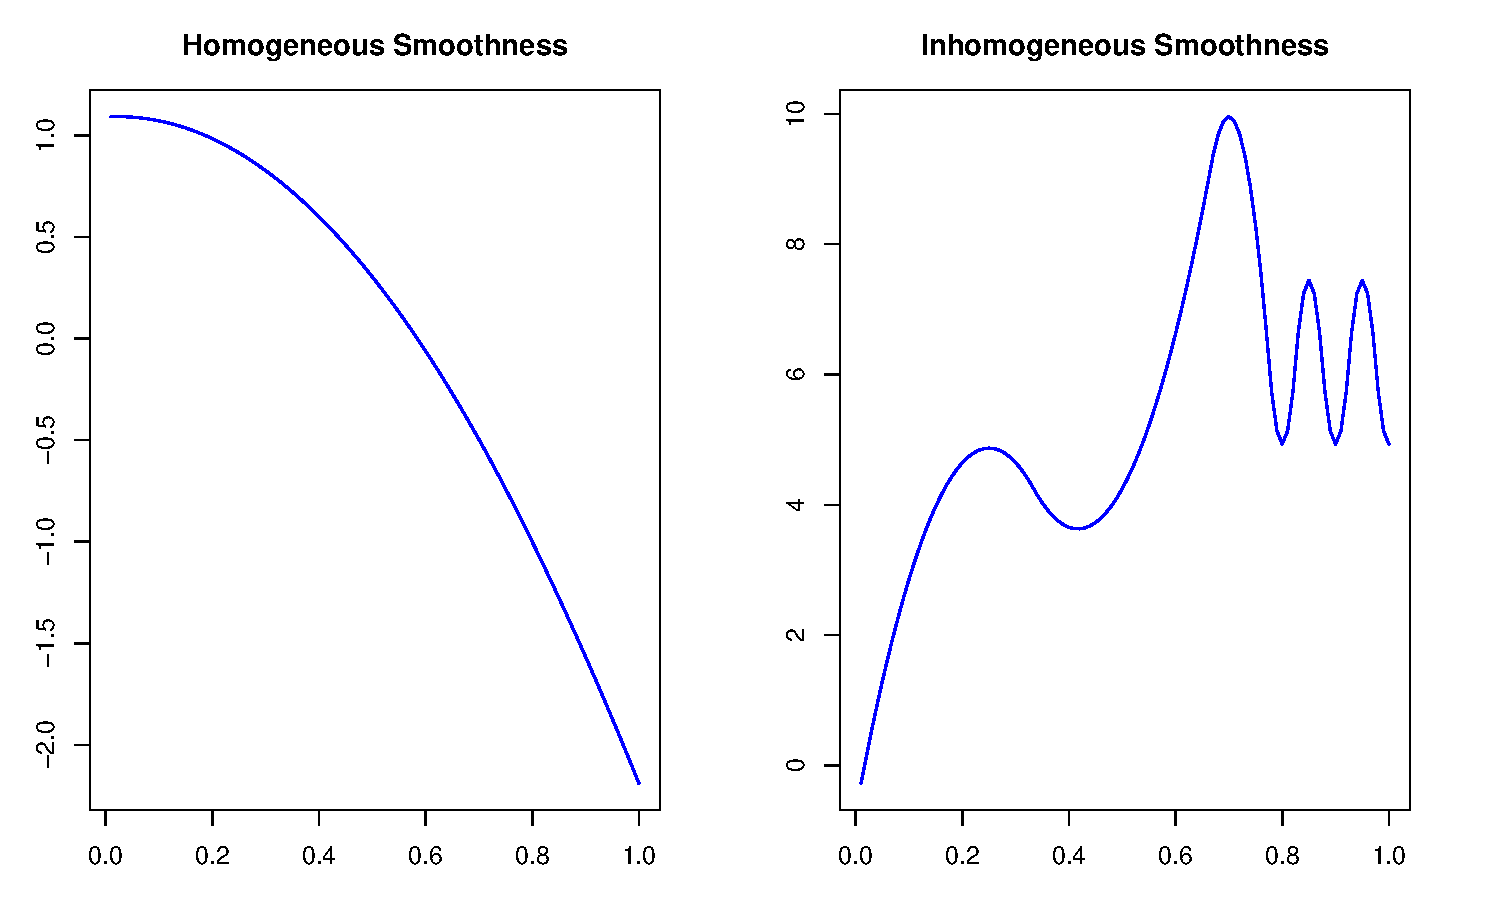
\includegraphics[width = 0.6\textwidth]{Figures/homo.pdf}
\caption{Examples of functions with homogeneous smoothness and inhomogeneous smoothness}
\label{fig:homo}
\end{figure}

From a theoretical point of view, linear smoother have been proved to be sub-optimal for certain function class. In nonparametric estimation, we don't assume a parametric form of the true function $f_0$, but rather have a milder assumption that $f_0$ lies in some smooth function. There are many notions of smoothness, some commonly used smooth function class include: H\"older class $H(k)$, Sobolev space $\cal{W}(k)$, total variation class $\cal{F}(k)$, where $k$ refers to the order of derivative. Rigorous definitions of these function classes will be deferred to Section \textcolor{red}{XXX}. One important result in minimax theory proved by \cite{donoho1998minimax} shows that under the $L_2$ risk, the minimax rate over the function class $\cal{F}(k)$ is $n^{-(2k+2)/(2k+3)}$, however when restricted to linear smoothers, the minimax rate is $n^{-(2k+1)/(2k+2)}$. This result demonstrated that linear smoothers are sub-optimal over functions with different orders of bounded variation. To make this more clear, if we assume the true function $f_0$ is of bounded variation, i.e. is in $\cal{F}(0)$, then the minimax convergence rate is $n^{-2/3}$, while any linear smoother can do no better than $n^{-1/2}$, which means linear smoothers will still be consistent but at a much slower rate. See Figure \ref{fig:diagram} for a convergence rate comparison for linear and nonlinear smoothers.

The above-mentioned defects of linear smoothers motivated the development of nonlinear smoothers. Before the technique of trend filtering was developed in this paper, two most effective nonlinear smoothers are wavelet smoothers\cite{johnstone2011gaussian,mallat2008wavelet,donoho1994ideal} and locally adaptive regression splines\cite{mammen1997locally}. Both methods have nice local adaptivity. In the top right panel of Figure \ref{fig:ssvslars}, we demonstrate the fit of locally adaptive splines, which is clearly better than the fit of smoothing splines. It nicely adapts to the "hills" on the right end while successfully maintaining the smoothness on the left end. Moreover, both methods have been proved to be minimax optimal over the total variation class. More specifically, \cite{donoho1998minimax} and \cite{mammen1997locally} respectively proved that wavelet methods and locally adaptive regression splines have minimax convergence rate $n^{-(2k+2)/(2k+3)}$, thus are optimal over the total variation class $\cal{F}(k)$. See Figure \textcolor{red}{XXX} for a diagram comparing the convergence rate of linear and nonlinear smoothers. These two methods are not perfect though. \textcolor{red}{For computational efficiency, wavelet methods require the inputs $(x_1,\ldots, x_n)$ to be evenly spaced, and sample size $n$ to be a power of 2, and there are often further assumptions made about the behavior of the fitted function at the boundaries of the input domain.} To solve the locally adaptive regression spline problem, on the other hand, there is no better alternative to solve a Lasso problem with dense design matrix $X$, which takes $\cal{O}(n^3)$ operations. Moreover, to choose the locations of the knots in locally adaptive regression spline is usually hard for spline of order $k\geq 2$. Limitations of wavelet methods and locally adaptive regression splines motivate us to look for a new nonlinear smoother, which is expected to be locally adaptive, computationally efficient and theoretically optimal in the minimax sense.

\begin{figure}[t!]
\centering
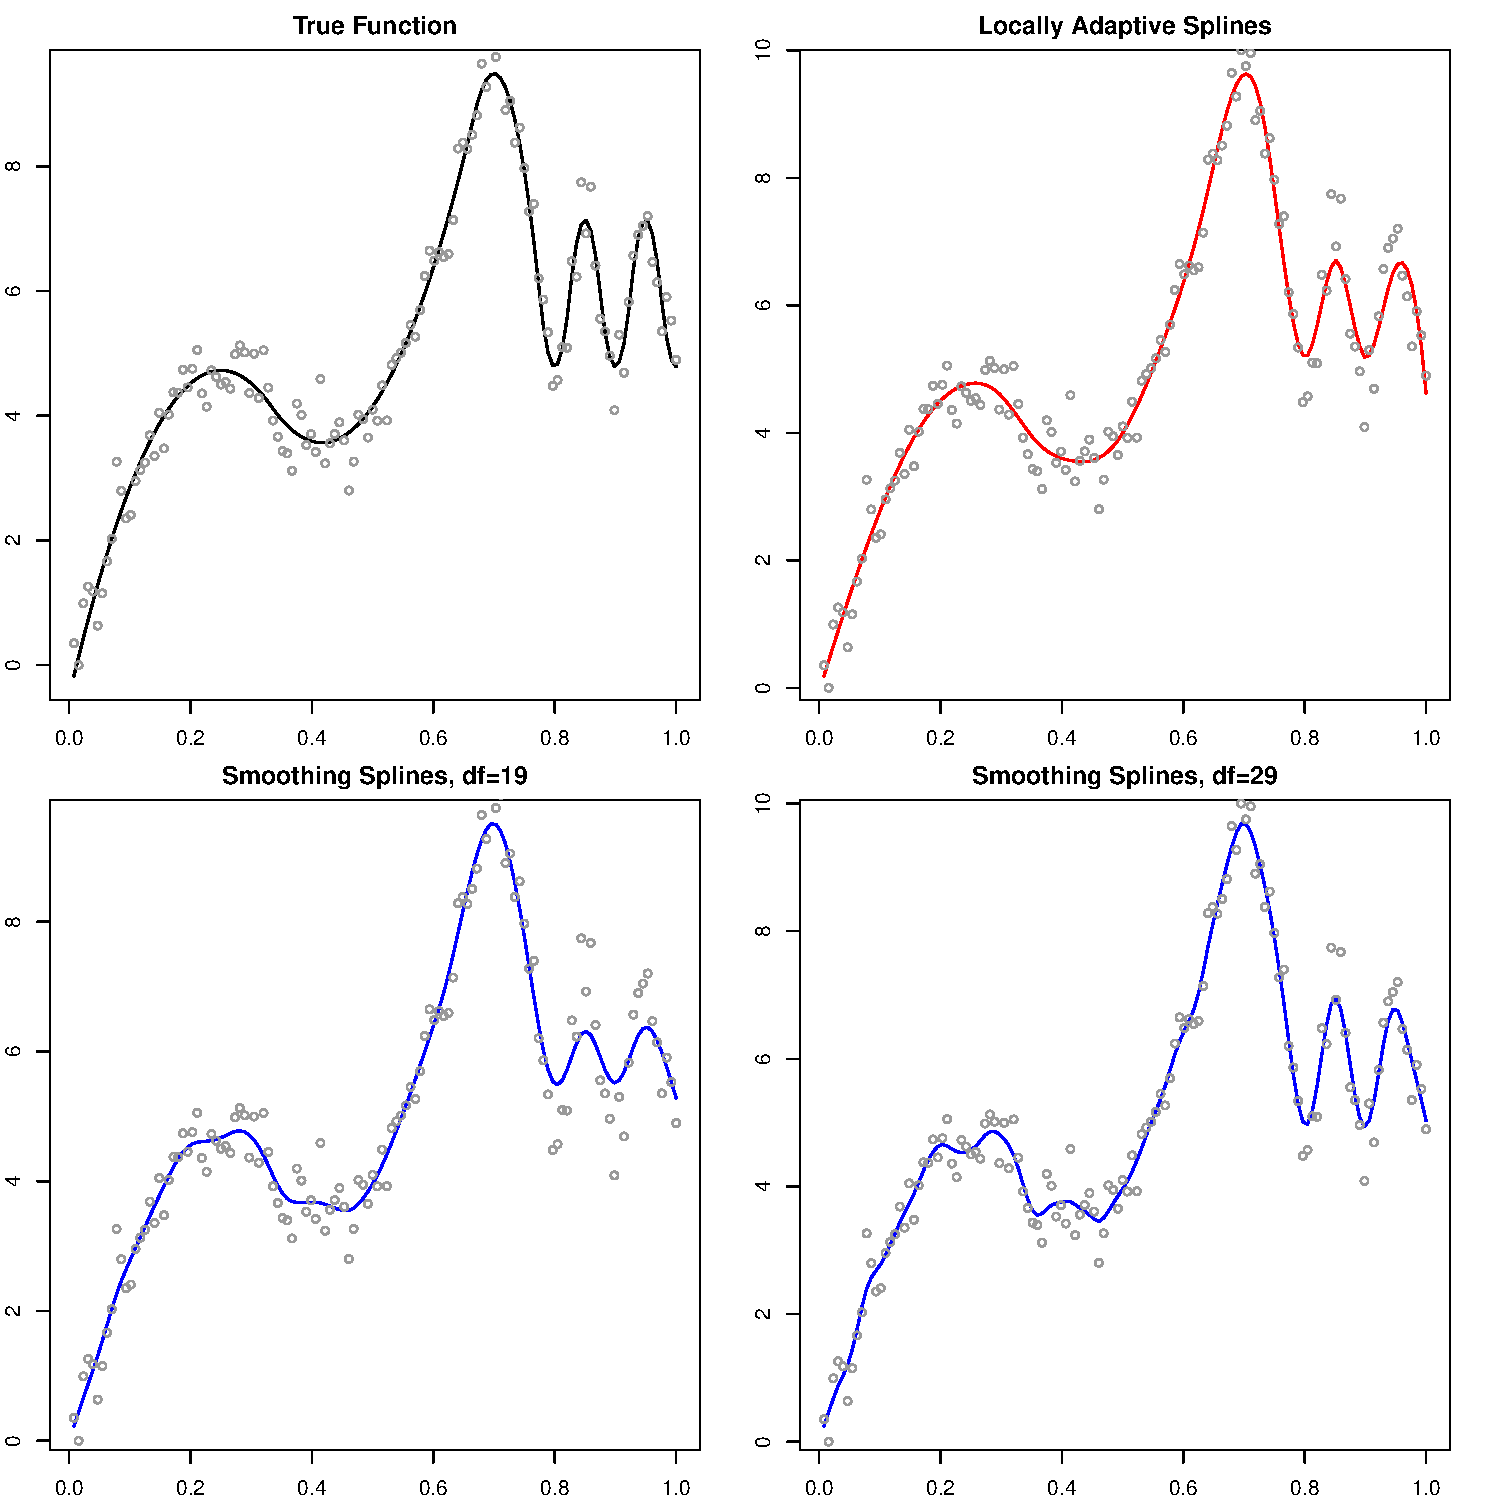
\includegraphics[width = 0.6\textwidth]{Figures/ssvslars.pdf}
\caption{Comparison of fit of smoothing splines and locally adaptive splines for true function with inhomogeneous smoothness}
\label{fig:ssvslars}
\end{figure}

In this paper, we will focus on one such method in the class of trend filtering estimators. Trend filtering, as its name suggests, was originally proposed to estimate the underlying trend in time series data, and had since then been applied in a variety of disciplines, such as economics (e.g. \cite{hodrick1997postwar,tsay2005analysis}), astronomy (e.g. \cite{kovacs2008application}), social science (e.g. \cite{saha2012learning,levitt2004understanding}), medical science (e.g. \cite{greenland1992methods,link1994estimating}), etc. Many methods for trend filtering have been proposed, including moving averaging smoothing (e.g. \cite{leser1961simple,kendall1946advanced,lucas1980two}), Hodrick-Prescott(H-P) filtering \cite{hodrick1997postwar},  smoothing splines (e.g. \cite{de1978practical,wahba1990spline,green1993nonparametric}). Most of the trend filtering techniques are based on $\ell_2$ regularization. H-P filtering, for example, directly penalizes the square of the second order difference of the fitted value for longitudinal data. A relatively new trend filtering technique based on $\ell_1$ norm was proposed in \cite{kim2009ell_1}, where the method solves the following optimization problem 

\begin{align}
\minimize_{u\in\RR^n} \frac{1}{2}\|y-u\|_2^2 + \lambda\sum_{i=2}^{n-1} |u_{i-1} - 2u_i + u_{i+1}|  \label{linear_tf}
\end{align}
where $y\in\RR^n$ is the observation signal of length $n$ and $\lambda$ is the tuning parameter. Unlike $\ell_2$ penalty, sparsity-inducing $\ell_1$ penalty of the discrete second-order difference will render certain entries to be zero and the fit will adapt to heterogeneous signals. The new trend filtering technique discussed in this paper is a natural extension of \eqref{linear_tf} and penalizes any order of discrete difference. Throughout the paper, we will work through and explore this more general version of $\ell_1$ trend filtering, and compare it with both linear and nonlinear smoothers. We will show that trend filtering is locally adaptive, can be solved by efficient algorithms and also has minimax convergence rate of $n^{-(2k+2)/(2k+1)}$ over the bounded total variation class $\cal{F}$.

\begin{figure}[t!]
\centering
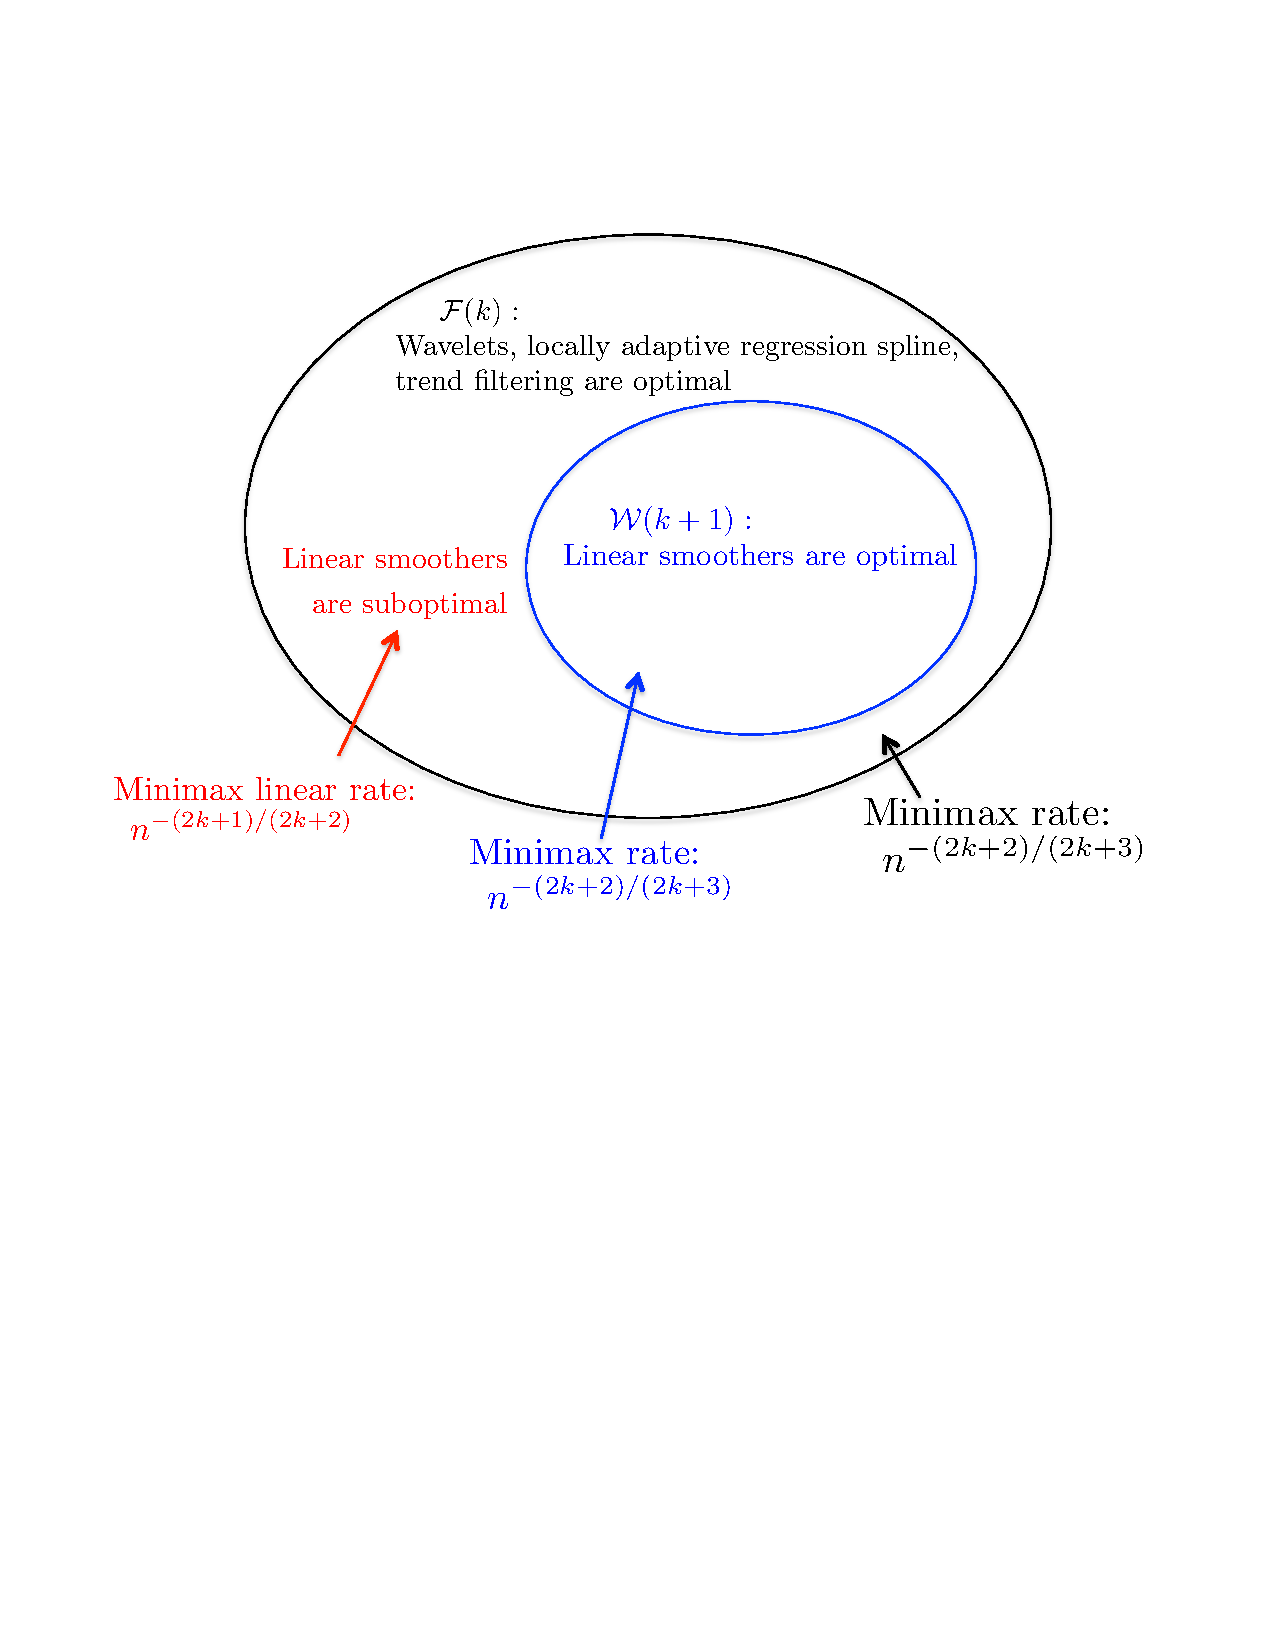
\includegraphics[width = 0.8\textwidth]{Figures/diagram.pdf}
\caption{Comparison of minimax convergence rate of linear smoothers and nonlinear smoothers}
\label{fig:diagram}
\end{figure}
 
It is worth mentioning that after this paper was published in 2014, there have been some exciting breakthroughs in the domain of trend filtering. \cite{wang2016trend} extends the notion of univariate trend filtering onto trend filtering on graphs and defines the discrete difference operator on graphs using the corresponding Laplacian matrix. \cite{sadhanala2017additive} and \cite{petersen2014fused} both extend trend filtering to high dimensions under the framework of additive model, while the latter focus on trend filtering with order $0$. \cite{wang2014falling} explores in depth the falling factorial basis used by the continuous-time representation of trend filtering. \cite{maidstone2017detecting} explores linear trend filtering ($k =1$) with $\ell_0$ penalty and proposes a novel dynamic-programming algorithm to solve the $\ell_0$ based optimization problem. 

The rest of the paper will be organized as follows. In Section 2, we will introduce the trend filtering model and discuss the corresponding algorithms to solve the minimization problem. We then compare trend filtering with smoothing splines and locally adaptive regression splines respectively in Section 3 and Section 4. In Section 5, we establish a continuous-time representation of trend filtering, which demonstrates the continuous version of the solution of trend filtering is piecewise polynomial. In Section 6, we derive the minimax convergence rate of trend filtering by linking it to locally adaptive regression splines. A real-data study is done in Section 7, followed by some discussion in Section 8 and a conclusion in Section 9. 


\section{Method}
\label{sec:method}

\subsection{Optimization Problem}
\label{subsec:opt_problem}
In this section, we generalize the $\ell_1$ trend filtering problem \eqref{linear_tf} into higher orders. The $k$-th order trend filtering is defined via the following optimization problem

\begin{align}
\minimize_{u\in\RR^n} \frac{1}{2}\|y-u\|_2^2 + \lambda\|D^{(k+1)}u\|_1  \label{tf}
\end{align}
where $\{y_1,\ldots, y_n\}$ are signal assumed to be observed at evenly-spaced time points $\{x_1,\ldots,x_n\}$, $\lambda$ is the tuning parameter, $D^{(k+1)}\in\RR^{(n-k-1)\times n}$ is the $(k+1)$-st order discrete derivative operator. For order $k = 0$, the difference operator $D^{(1)}$ in \eqref{tf} is defined as

\begin{align}
D^{(1)} =
\begin{bmatrix}
-1 & 1 & 0 & \ldots & 0 & 0\\
0 & -1 & 1 & \ldots & 0 & 0\\
\vdots & \vdots & \vdots & \ddots & \vdots & \vdots\\
0 & 0 & 0 & \ldots & -1 & 1
\end{bmatrix}\in\RR^{(n-1) \times n}
\end{align}
and therefore the penalty term in \eqref{tf} becomes $\lambda\sum_{i=1}^{n-1}|u_{i+1}- u_i|$. This coincides with 1-dimensional total-variation denoising \cite{rudin1992nonlinear,harchaoui2010multiple} and also the fused-lasso problem with only the fused penalty term \cite{tibshirani2005sparsity}. When $k = 1$, the discrete difference operator $D^{(2)}$ becomes


\begin{align}
D^{(2)} =
\begin{bmatrix}
1 & -2 & 1 & 0 & \ldots & 0 & 0\\
0 & 1 & -2 & 1 & \ldots & 0 & 0\\
\vdots & \vdots & \vdots & \ddots & \vdots & \vdots & \vdots\\
0 & 0 & 0 & \ldots & 1 & -2 & 1
\end{bmatrix}\in\RR^{(n-2) \times n}
\end{align}



Without surprise, this recovers the linear trend filtering defined in \eqref{tf}. For $k\geq 2$, the difference operator is defined recursively by 

\begin{align}
D^{(k+1)} \equiv D^{(1)} \cdot D^{(k)} \label{difference_op}
\end{align}
thus the $(k+1)$-st difference operator penalizes the change in the $k$-th order difference. Under the assumption that $\{y_1,y_2,\ldots, y_n\}$ are observed at evenly-spaced time points $\{x_1,x_2,\ldots, x_N\}$, the definition in \eqref{difference_op} mimics the definition of derivatives and could be seen as a discrete version of derivatives. One might accordingly expect the $k$-th order trend filtering estimator to behave somewhat similar to the piecewise $k$-th order polynomials. Figure \ref{fig:Figure1_examples} gives some empirical evidences of this claim. From left to right, data are generated from the piecewise constant, piecewise linear and piecewise quadratic true function, and correspondingly we fit trend filtering of order $k = 0,1,2$ at certain tuning parameter $\lambda$. Note that the solution to \eqref{tf} is only defined on the observed points $\{x_1,x_2, \ldots, x_n\}$, but we use linear interpolation to display a "continuous" version of trend filtering. The "continuous" version do seem like piecewise constant, piecewise linear and piecewise quadratic for their corresponding orders. So a natural question arises: is there a continuous representation $f(x)$ of trend filtering, e.g. the solution $\{\hat{u}_1,\ldots, \hat{u}_n\}$ to \eqref{tf} are evaluations of $f$ at $\{x_1, x_2,\ldots, x_n\}$. And if there is, if $f$ indeed a piecewise polynomial or spline? (Recall that $k$-th order splines are $k$-th order piecewise polynomials with extra requirements of continuous derivatives up to order $k-1$). For the first question, the answer is yes, and we will develop a continuous time representation of trend filtering in Section \textcolor{red}{XXX}. For the second question, we will also prove in Section \textcolor{red}{XXX} that for $k=0$ and $k=1$, the continuous representation of trend filtering are indeed splines, but for $k\geq 2$, the solution is piecewise polynomial but not spline. 

\begin{figure}[t!]
\centering
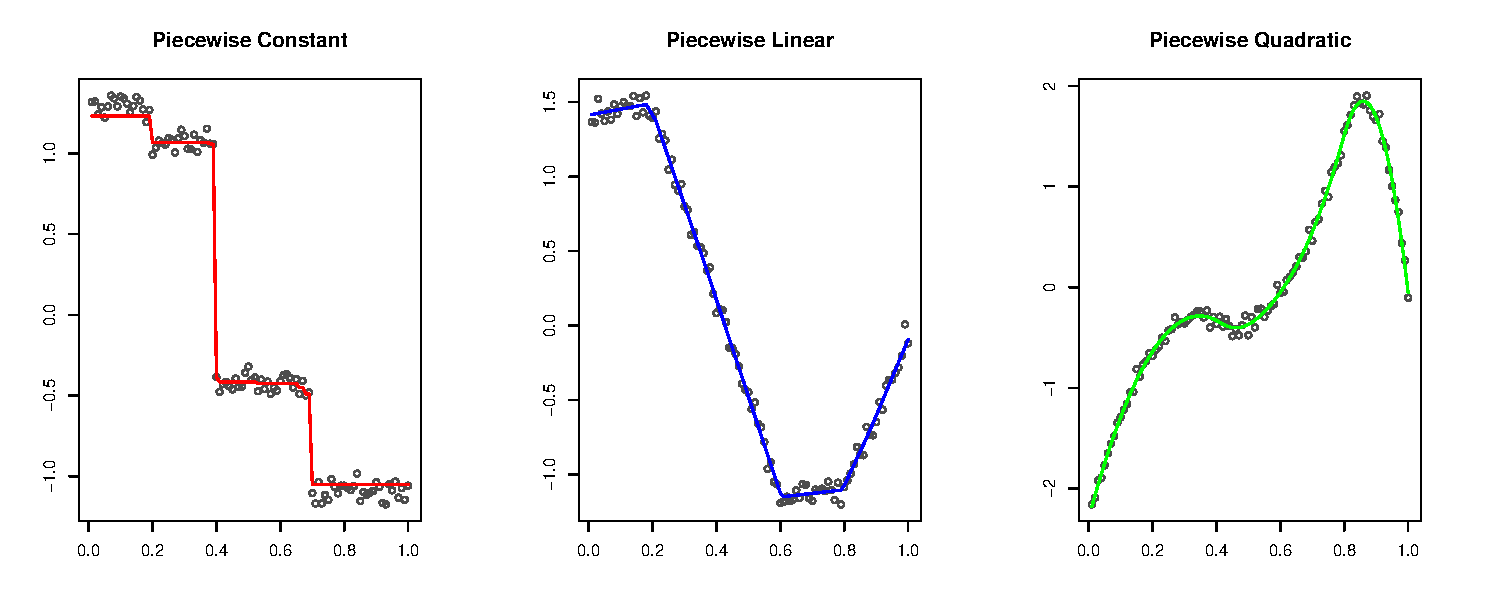
\includegraphics[width = 0.8\textwidth]{Figures/Figure1.pdf}
\caption{Examples of trend filtering fits of order $k =0, 1, 2$. The solution to \eqref{tf} are only defined on the input points $x_i = i/n$ wit h $i=1,2,\ldots, n$, but we use linear interpolation to display a "continuous" version of trend filtering.}
\label{fig:Figure1_examples}
\end{figure}

\subsection{Trend Filtering as Lasso Type Problem}
\label{subsec:tfaslasso}
For the rest of the section, we will discuss some properties of trend filtering. Consider the generalized lasso problem defined as

\begin{align}
\minimize_{\beta\in\RR^p} \frac{1}{2}\|y-X\beta\|_2^2 + \lambda\|D\beta\|_1 \label{eq:genlasso}
\end{align}
where $D\in\RR^{r\times p}$ is some specified penalty matrix. In contrast to the ordinary Lasso problem, which directly penalizes the absolute value of the entries of $\beta$, the generalized Lasso induces sparsity of $D\beta$ to satisfy some desired behavior of $\beta$. By comparing \eqref{tf} with \eqref{eq:genlasso}, we can see that $k$-th order trend filtering is also a generalized lasso problem with design matrix $X = \mathbb{I}_n$ and penalty matrix $D = D^{(k+1)}$, which indicates trend filtering enjoys many generalized Lasso properties. One of the properties of interest is the degree of freedom, which we will use as a metric for model complexity to compare with other methods in later sections. \cite{tibshirani2011solution} fully characterizes the degree of freedom in Lasso-type problem, and proves that one unbiased estimator of the degree of freedom for \eqref{tf} is



\begin{align}
\mbox{df}(\hat{u}) = \|D^{(k+1)}\hat{u}\|_0 + k + 1 \label{eq:dof}
\end{align}
where $\|\cdot\|_0$ is the number of nonzero entries. Note that $D^{(k+1)}$ takes the difference of $k$-th order discrete difference, thus nonzero entries in $D^{(k+1)}\hat{u}$ correspond to knots or change points in the $k$-th order discrete difference. \eqref{eq:dof} might seem strange in the first place, because the fit of $k$-th order regression splines with the same knots has the same degree of freedom. Intuitively, trend filtering should have a larger degree of freedom compared to regression splines because it also spends some degrees of freedom to locate those knots. However, the shrinkage of $D\hat{\beta}$ to zero in \eqref{eq:genlasso} counterbalances the extra degrees of freedom spent on the search, and the resulting degree of freedom is the same as the corresponding equality-constrained least square estimates. Such phenomenon is called the "over-shrinkage" property and also exists for ordinary Lasso. Figure \ref{fig:Figure2_overshrinkage} compares trend filtering fit with corresponding regression splines with the same knots. The left and right panel fit a linear and cubic trend filtering respectively, and correspondingly piecewise linear and piecewise cubic regression splines with the same knots. The knots are marked with vertical dashed lines. We can see from the left panel that at the knots, regression spline is making a greater change of slope compared with trend filtering. On the right panel, regression spline also displays larger curvature on the left and right half separated by the knot. A closer look at different orders of discrete difference of trend filtering is shown in Figure \ref{fig:Figure3_discrete}. Again this empirically justifies the claim that the continuous representation of trend filtering is $k$-th order piecewise polynomial because only the $3$rd order derivative of cubic trend filtering is discontinuous and it is constant on the two segments separated by the knot.  

\begin{figure}[t!]
\centering
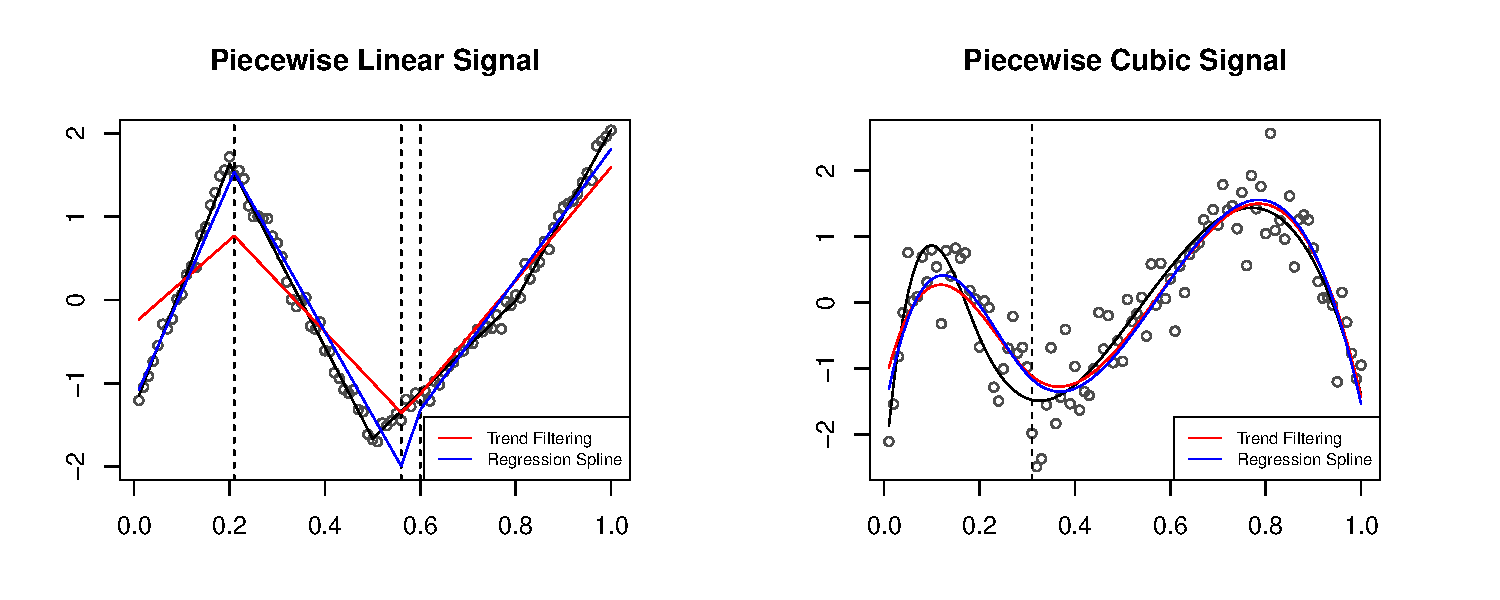
\includegraphics[width = 1.0\textwidth]{Figures/Figure2.pdf}
\caption{Comparison of trend filtering and regression splines with the same knots to demonstrate the over-shrinkage nature of generalized Lasso.}
\label{fig:Figure2_overshrinkage}
\end{figure}


\begin{figure}[t!]
\centering
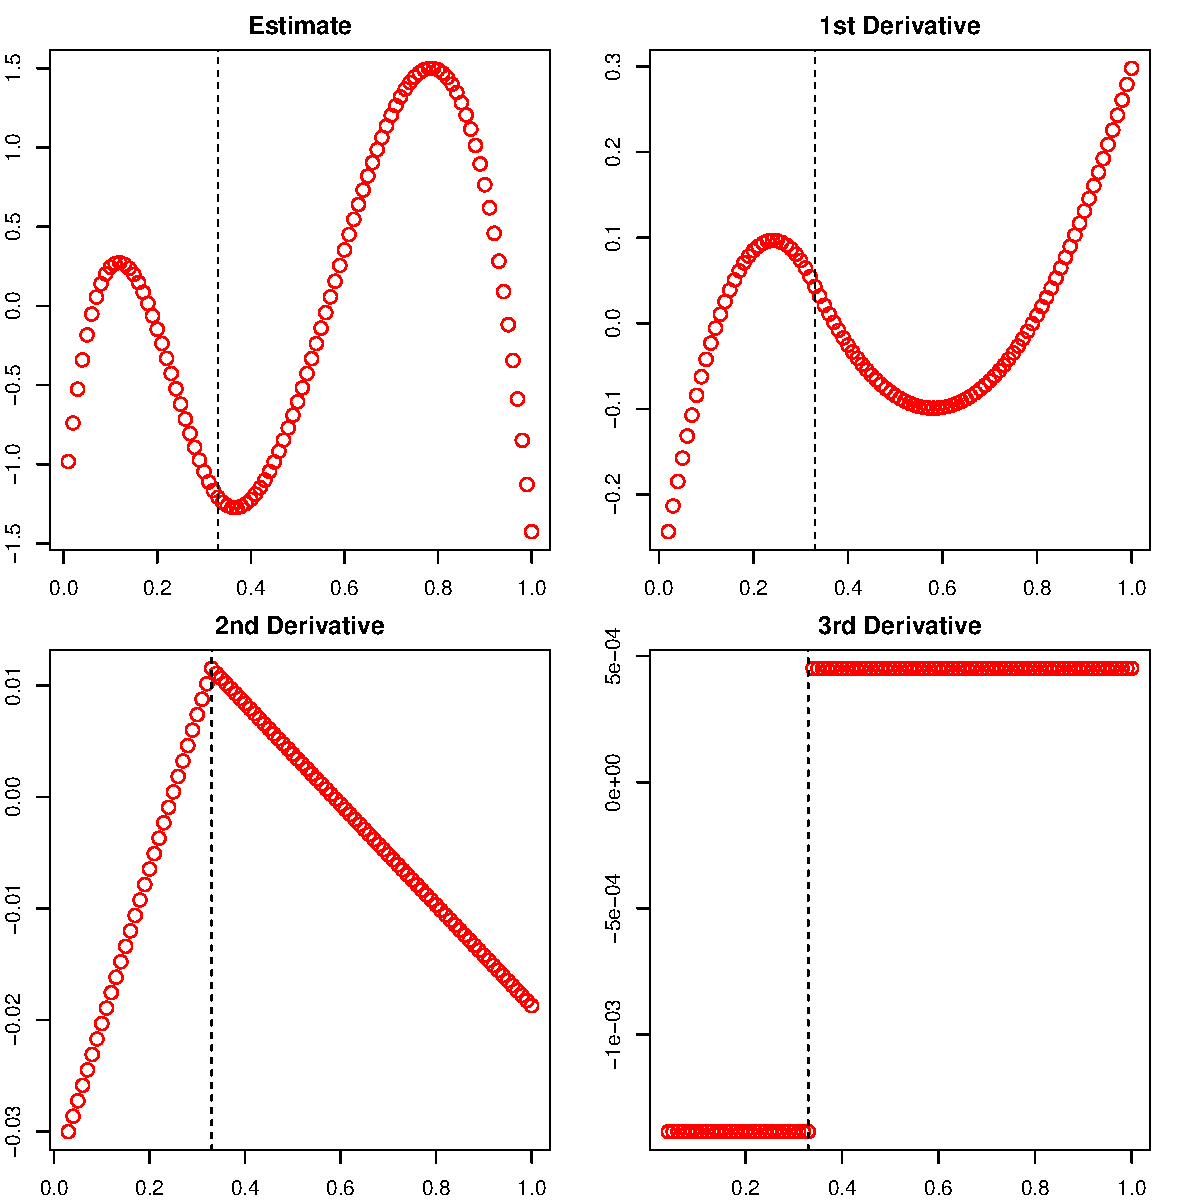
\includegraphics[width = 0.6\textwidth]{Figures/Figure3.pdf}
\caption{Different orders of discrete difference of cubic trend filtering. Each order of discrete difference is computed by $D^{(k+1)}\hat{u}$ for $k=0,1,2$, where $\hat{u}$ is the solution to \eqref{tf}.}
\label{fig:Figure3_discrete}
\end{figure}

\eqref{eq:genlasso} shows that trend filtering can be posed as a generalized Lasso problem. Notice the penalty matrix $D=D^{(k)}$ in trend filtering is a wide matrix, i.e. $D^{(k)}$ has more rows than columns and more importantly $D^{(k)}$ has full column rank for all orders of trend filtering. This enables us to invert the penalty matrix and rewrite trend filtering as an ordinary Lasso problem. More accurately, we have

\begin{lemma}
The trend filtering problem \eqref{tf} is equivalent to the following Lasso problem
\begin{align}
\hat{\alpha} = \argmin_{\alpha\in\RR^n}\frac{1}{2}\|y-H\alpha\|_2^2 + \lambda\sum_{j=k+2}^n |\alpha_j|
\label{eq:tf_lasso}
\end{align}
in that the solution satisfies $\hat{u} = H\hat{\alpha}$. Here the design matrix $H\in\RR^n$ is given by
\begin{equation}
H_{ij} = 
\begin{cases}
(\frac{i}{n})^{j-1}, & \text{for } i = 1,\ldots, n, j=1,\ldots, k+1\\
0, & \text{for } i \leq j-1, j\geq k+2\\
\sigma_{i-j+1}^{(k)} \cdot k!/n^k, &\text{for } i > j-1, j\geq k+2
\end{cases}
\label{eq:H_cumsum}
\end{equation}
where $\sigma_i^{(0)} = 1$ for all $i$ and
\begin{align*}
\sigma^{(k)}_i = \sum_{j=1}^i \sigma_j^{(k-1)}
\end{align*}
that is $\sigma_i^{(k)}$ is the $k$th order cumulative sum of $(1,1,\ldots, 1)\in\RR^i$.
\end{lemma}
It is worth mentioning that \eqref{eq:tf_lasso} is a generalization for the case $k =1$ in Section 3.2 of \cite{kim2009ell_1}. Notice that the design matrix in \eqref{eq:tf_lasso} is close to a lower-triangular matrix and thus has a sparse structure, which makes general lasso solver very efficient for solving \eqref{eq:tf_lasso}. We will compare the Lasso solver with two other algorithms in Section \ref{subsec:algo}. 

\subsection{Continuous Representation of Trend Filtering}
\label{subsec:ct_tf}
Note that the solution $\hat{u}$ to \eqref{tf} is just discrete values at the input $(x_1,\ldots, x_n)$ but doesn't tell us the exact form of our estimator $\hat{f}$ of the true regression function $f_0$. This will be problematic if we want to predict the value of $f_0$ at points outside the input. This motivates us to think about the following question: given the equivalent Lasso form \eqref{eq:tf_lasso} of trend filtering, is there a set of basis functions whose evaluations at the input $(x_1,\ldots, x_n)$ give the design matrix $H$? The following lemma gives an affirmative answer.

\begin{lemma}
For evenly-spaced points $(x_1,\ldots, x_n)$ with $x_i = \frac{i}{n}$ for $i=1,\ldots, n$, define the set of functions $(h_1, \ldots, h_n)$ such that
\begin{equation}
\begin{aligned}
h_1(x) = 1, \quad h_2(x) = x, \ldots, h_{k+1}(x) = x^k,\\
h_{k+1+j}(x) = \prod_{l=1}^k (x-x_{j+l})\mathbbm{1}_{[x\geq x_{j+k}]}, \quad \text{for } j = 1,\ldots, n-k-1
\label{eq:fall_fact}
\end{aligned}
\end{equation}
Then the design matrix $H$ in \eqref{eq:tf_lasso} is evaluations of $(h_1,\ldots, h_n)$ at $(x_1,\ldots, x_n)$, i.e.
\begin{align*}
H_{ij} = h_j(x_i) \quad i,j=1,\ldots, n
\end{align*}
\end{lemma}
Note that the basis functions $(h_1,\ldots, h_n)$ defined by \eqref{eq:fall_fact} are piecewise polynomial functions up to order $k$. Consider the truncated power basis of the same order defined on $x_i = \frac{i}{n}$ for $i= 1,\ldots, n$,
\begin{equation}
\begin{aligned}
g_1(x) = 1, \quad g_2(x) = x, \ldots, g_{k+1}(x) = x^k,\\
g_{k+1+j}(x) = (x-x_j)^k\mathbbm{1}_{[x\geq x_j]}, \quad \text{for }j=1,\ldots, n-k-1
\label{eq:trun_basis}
\end{aligned}
\end{equation}


\begin{figure}[t!]
\centering
   \begin{subfigure}[b]{1\textwidth}
   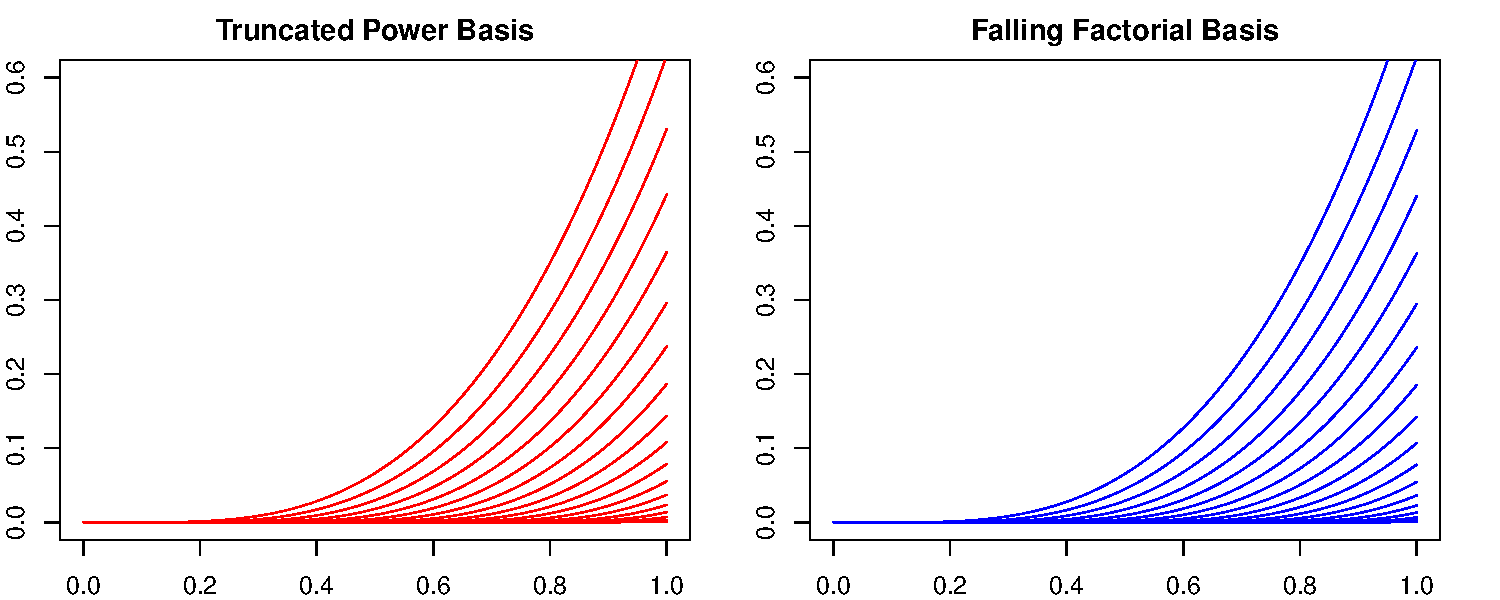
\includegraphics[width=1\linewidth]{Figures/Figure8.pdf}
   \caption{}
\end{subfigure}

\begin{subfigure}[b]{1\textwidth}
   \includegraphics[width=1\linewidth]{Figures/Figure8b.pdf}
   \caption{}
\end{subfigure}

\caption[Two numerical solutions]{(a) Comparison of truncated power basis and falling factorial basis of order $k=3$. The left panel shows the truncated power basis \eqref{eq:trun_basis} and the right panel shows the falling factorial basis \eqref{eq:fall_fact}. Both sets of basis functions are defined over evenly-spaced $x_i = \frac{i}{n}$ for $i=1,\ldots, n$ with $n = 22$. Visually these two sets of functions are very similar. (b) Zoomed in parts of truncated power basis and falling factorial basis with same order and knots as (a). The left panel zooms in truncated power basis and the right panel zooms in the falling factorial basis. Truncated power basis has continuous derivative up to order 2, but the falling factorial basis has discontinuous first and second order derivatives.}
\label{fig:Figure8_fall}
\end{figure}


% \begin{figure}[t!]
% \centering
% 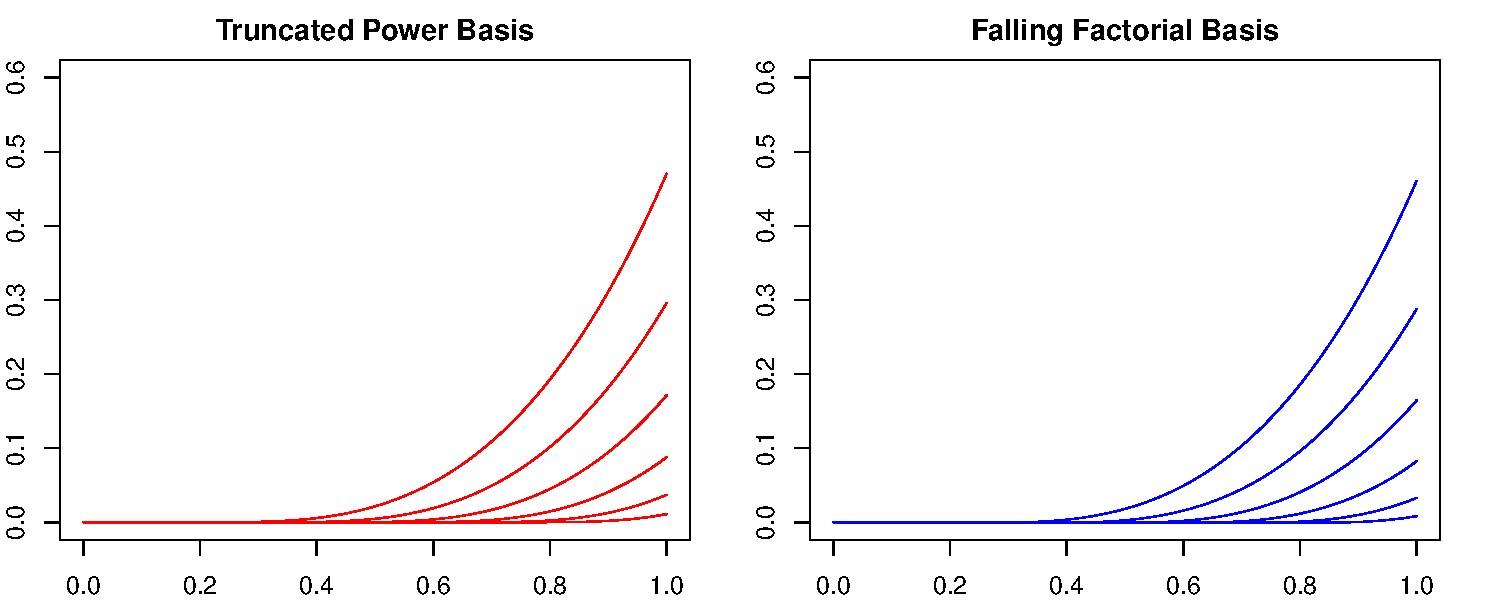
\includegraphics[width = 1\textwidth]{Figure8.pdf}
% \caption{Comparison of truncated power basis and falling factorial basis of order $k=3$. The left panel shows the truncated power basis \eqref{eq:trun_basis} and the right panel shows the falling factorial basis \eqref{eq:fall_fact}. Both sets of basis functions are defined over evenly-spaced $x_i = \frac{i}{n}$ for $i=1,\ldots, n$ with $n = 22$. Visually these two sets of functions are very similar.}
% \label{fig:Figure8_fall}
% \end{figure}

% \begin{figure}[t!]
% \centering
% \includegraphics[width = 1\textwidth]{Figure8b.pdf}
% \caption{Zoomed in parts of truncated power basis and falling factorial basis with same order and knots as Figure \ref{fig:Figure8_fall}. The left panel zooms in truncated power basis and the right panel zooms in the falling factorial basis. Truncated power basis has continuous derivative up to order 2, but the falling factorial basis has discontinuous first and second order derivatives.}
% \label{fig:Figure8b_fall}
% \end{figure}


Comparing \eqref{eq:fall_fact} and \eqref{eq:trun_basis}, we can see that these two sets of functions are extremely similar. In fact, the function set \eqref{eq:fall_fact} is called the falling factorial basis\cite{wang2014falling}, because each $h_{k+1+j}$ is the "falling" substitute of $g_{k+1+j}$ by replacing $(x-x_j)(x-x_j)\ldots(x-x_j)$ with $(x-x_{j+1})(x-x_{j+2})\ldots(x-x_{j+k})$. The upper panel of Figure \ref{fig:Figure8_fall} compares the truncated power basis and falling factorial basis of order $k = 3$. Both sets of functions are defined over evenly-spaced knots $x_i = \frac{i}{n}$ for $i= 1,\ldots, n$ with $n = 22$. We can see visually they are very similar. There is one nontrivial difference between these two sets though. It is well known that the $k$th order truncated power basis is basis for regression splines, which means each $g_i$ for $i=1,\ldots, n$ are $k$th order piecewise polynomial with continuous derivative up to order $k-1$. However, this is not true for the falling factorial basis. The lower panel of Figure \ref{fig:Figure8_fall} zooms in parts of both basis sets. With $k =3$, truncated power basis has continuous 1st and 2nd order derivative, while falling power basis is continuous but has discontinuous first two derivatives.

The following lemma adopts the falling factorial basis \eqref{eq:fall_fact} to define a continuous representation of trend filtering:
\begin{lemma}
For inputs $x_1<\ldots<x_n$ and the basis functions $(h_1,\ldots, h_n)$ defined in \eqref{eq:fall_fact}, define the linear subspace of functions
\begin{align}
\cal{H}_k = \text{span}\{h_1,\ldots, h_n\} = \Big\{\sum_{j=1}^n \alpha_jh_j:\alpha_1,\ldots, \alpha_n\in\RR\Big\}
\label{eq:linear_class}
\end{align}
If the inputs are evenly-spaced, $x_i=\frac{i}{n}$ for $i=1,\ldots, n$, then the continuous minimization problem
\begin{align}
\hat{f} = \argmin_{f\in\cal{H}_k} \frac{1}{2}\sum_{i=1}^n(y_i-f(x_i))^2 + \lambda\cdot\text{TV}(f^{(k)})
\end{align}
is equivalent to the trend filtering problem \eqref{tf} in that their solutions are the same at inputs.
\begin{align*}
\hat{u}_i = \hat{f}(x_i) \quad \text{for } i=1,\ldots,n  
\end{align*}
\label{lemma:cont}
\end{lemma}

Despite the original formulation of trend filtering in \eqref{tf} is discrete in nature, Lemma \ref{lemma:cont} nicely characterizes a continuous representation of trend filtering, which facilitates the comparison with other function estimation technique, such as smoothing spline and locally adaptive regression spline. Moreover, since the falling factorial basis \eqref{eq:fall_fact} has discontinuous lower-order derivative for $k\geq 2$, we conclude that for $k = 0,1$, the continuous representation of trend filtering generates a fit that is constant spline or linear spline respectively; for $k\geq 2$, the fit of continuous trend filtering is piecewise polynomial but not spline.

\subsection{Algorithms}
\label{subsec:algo}
The Lasso form \eqref{eq:tf_lasso} and generalized Lasso form \eqref{eq:genlasso} of trend filtering motivate at least three efficient algorithms. 

\textbf{Algorithm I} The first algorithm solves the Lasso problem \eqref{eq:tf_lasso}. Notice that \eqref{eq:tf_lasso} is not a standard Lasso problem because the $\ell_1$ penalty does not penalize the first $(k+1)$ entries. However, we could first solve the first $(k+1)$ entries in terms of the rest, then solve the standard Lasso problem. More specifically, write $H = [H_1,H_2], \alpha = [\alpha_1, \alpha_2]$, such that $H_1$ and $\alpha_1$ refers to the first $(k+1)$ columns of $H$ and first $(k+1)$ entries of $\alpha$ respectively. Now take the derivative of the objective function in \eqref{eq:tf_lasso} with respect to $\alpha_1$ and set it to zero, we obtain

\begin{align}
\hat{\alpha}_1 = (H_1^TH_1)^{-1}H_1^T(y-H_2\alpha_2) 
\label{eq:algo_lasso}
\end{align}

Now plug \eqref{eq:algo_lasso} into \eqref{eq:tf_lasso}, we obtain the standard-form Lasso problem

\begin{align}
\hat{\alpha}_2 = \argmin_{\alpha_2\in\RR^{n-k-1}} \frac{1}{2}\|\tilde{y} - \tilde{X}\alpha_2\|_2^2 + \lambda\|\alpha_2\|_1
\label{eq:algo_lasso2}
\end{align}
where $\tilde{y} \equiv (\mathbb{I}_n - H_1(H_1^TH_1)^{-1}H_1^T)y$ and $\tilde{X} \equiv (\mathbb{I}_n - H_1(H_1^TH_1)^{-1}H_1^T)H_2$. The solution for \eqref{eq:tf_lasso} becomes 
\begin{align}
\hat{\alpha} = ((H_1^TH_1)^{-1}H_1^T(y-H_2\hat{\alpha}_2), \hat{\alpha}_2)
\end{align}
The computational cost for solving $\alpha_1$ is $\cal{O}(nk^2)$, and solving Lasso problem \eqref{eq:algo_lasso2} using, for example, least angle regression\cite{efron2004least} requires $\cal{O}(k^3 + nk+2)$. For $k\leq n$, this requires $\cal{O}(nk^2)$ operations in total to solve the trend filtering problem for one $\lambda$. The \textit{lars} R package solves \eqref{eq:algo_lasso} for all $\lambda$ values and the \textit{glmnet} R package solves \eqref{eq:algo_lasso2} for a sequence of $\lambda$ values.

\textbf{Algorithm II} The second algorithm is the path algorithm for solving generalized Lasso problem \eqref{eq:genlasso}, proposed in \cite{harchaoui2010multiple,tibshirani2011solution}. This algorithm solves the dual problem of \eqref{eq:genlasso}, which after some simple algebra gives

\begin{equation}
\begin{aligned}
&\minimize_{u\in\RR^m} \frac{1}{2}\|y-D^Tu\|_2^2\\
&\mbox{subject to } \|u\|_\infty \leq \lambda
\label{eq:algo_dual}
\end{aligned}
\end{equation}
where $m$ is the number of rows of $D$. The path algorithm starts from $\lambda = \infty$ and solves \eqref{eq:algo_dual} for all $\lambda$ values. The solution $\hat{u}_\lambda$ indexed by $\lambda$ is a piecewise linear function with respect to $\lambda$. The computational cost for each critical point in the path is $\cal{O}(n)$. However, in practice, the path algorithm may take number of critical points much larger than $n$ to converge. The \textit{genlasso} R packages provides efficient implementation of this algorithm.

\textbf{Algorithm III} The third algorithm also solves the dual problem \eqref{eq:algo_dual} instead of the primal problem, using an interior point algorithm. Such algorithm was first proposed in \cite{kim2009ell_1} to solve linear trend filtering problem but can be easily extended to solve higher order problems. Each iteration of the primal-dual interior point algorithm takes $\cal{O}(n)$ operations and the worst-case scenario takes $\cal{O}(n^{1/2})$ iterations, thus the worst-case overall computation cost is $\cal{O}^{3/2}$ to solve for a single $\lambda$. However, the authors report that in practice the number of iterations is only a few tens and is nearly independent of the sample size $n$, thus the practical computation cost is close to $\cal{O}(n)$. Efficient implementation in C and Matlab can be found at \url{http://stanford.edu/~boyd/l1_tf}. 

Since the most commonly used order for trend filtering is $k = 3$, we compare the performance of Algorithm I using the \textit{lars} R package and Algorithm II using the \textit{trendfilter} function in \textit{genlasso} package. We test the case with $n = 1000$, on a standard laptop, Algorithm I takes about 14 seconds for $4018$ $\lambda$ values, and Algorithm II takes 19 seconds for $4239$ critical points. The \textit{lars} package is relatively faster. 


\section{Comparison with Smoothing Spline}
\label{sec:comp_ss}
Smoothing spline is an extremely popular tool in nonparametric function estimation. It has more flexibility compared to regression spline because it circumvents the problem of knot selection(as they just use the inputs as knots). Smoothing spline was originally motivate and defined from a functional minimization perspective. Given inputs $(x_1,\ldots, x_n)$ lying in an interval, say $[0, 1]$, the smoothing spline estimate $\hat{f}$ of a given odd integer order $k\geq 0$ is defined as

\begin{align}
\hat{f} = \argmin_{f\in\cal{W}_{(k+1)/2}}\sum_{i=1}^n (y_i - f(x_i))^2 + \lambda \int_0^1 (f^{((k+1)/2)}(t))^2dt
\label{eq:ss}
\end{align}
where $f^{((k+1)/2)}(t)$ the $(k+1)/2$th order derivative of $f$ and the function class $\cal{W}_{(k+1)/2}$ is the $((k+1)/2)$nd order Sobolev space defined as

\begin{align*}
\cal{W}_{(k+1)/2} = \big\{f:[0,1]\rightarrow \RR:f\text{ is (k+1)/2 times differentiable with } \int_0^1(f^{((k+1)/2)}(t))^2dt<\infty\big\}
\end{align*}
\eqref{eq:ss} is an infinite-dimensional optimization problem over all functions $f$ in the $((k+1)/2)$nd order Sobolev space. This optimization criterion trades off the least squares error of $f$ over the observed pairs $(x_i, y_i)$, $i=1,\ldots, n$, with a penalty term that is large when the $((k+1)/2)$nd derivative of $f$ is wiggly. The tuning parameter $\lambda \geq 0$ governs the strength of each term in the minimization. Note that in order for the definition \eqref{eq:ss} to be valid, $k$ must be an odd integer. In practice, the most commonly used order is $k = 3$, i.e. cubic smoothing spline. 

Despite the infinite-dimensional nature in \eqref{eq:ss}, we will show in the next paragraph that smoothing spline has the so called \textit{variational} property. Roughly speaking, this property indicates that the best interpolant of \eqref{eq:ss}, i.e. the function with the smallest derivative penalty $\int_0^1(f^{((k+1)/2)}(t))^2dt$ among all those matching function values at inputs $(x_1,\ldots, x_n)$ is a natural spline of order $k$ with knots located at each distinct value of $(x_1,\ldots, x_n)$. This remarkable property of smoothing spline renders \eqref{eq:ss} finite-dimensional and makes computation for smoothing spline extremely efficient.

\subsection{Variational Property}
\label{subsec:var_property}
It can be proved[see Exercise 5.7 of \cite{friedman2001elements}] that the solution to \eqref{eq:ss} is a natural spline of order $k$ with knots located at distinct values of $(x_1,\ldots, x_n)$. This is called the \textit{variational} property of smoothing spline\cite{anselone1968general}. Easy calculation shows that the space of $k$th order natural spline has $n$ basis functions. Consider such a basis $(\eta_1,\ldots, \eta_n)$, let matrix $N\in\RR^{n\times n}$ be the evaluation of $\eta_1,\ldots, \eta_n$ at inputs $(x_1,\ldots, x_n)$ and $\Omega$ contains the integrated products of the $((k+1)/2)$nd order derivative of $(\eta_1,\ldots, \eta_n)$, i.e.
\begin{align}
N_{ij} = \eta_j(x_i), \quad \Omega_{ij} = \int_0^1 \eta_i^{((k+1)/2)}(t)\eta_j^{((k+1)/2)}(t)dt \quad i,j=1,\ldots,n
\label{eq:ss_N}
\end{align}
then the infinite-dimensional problem \eqref{eq:ss} can be written more succinctly as

\begin{align}
\hat{\beta} = \argmin_{\beta\in\RR^n} \|y-N\beta\|_2^2 + \lambda\beta^T\Omega\beta
\label{eq:ss_ridge}
\end{align}
showing the smoothing spline problem to be a type of generalized ridge regression problem. In fact, \eqref{eq:ss_ridge} has the closed-form solution
\begin{align}
\hat{\beta} = (N^TN + \lambda\Omega)^{-1}N^Ty
\end{align}
and therefore the fitted values $\hat{\mu} = (\hat{f}(x_1),\ldots, \hat{f}(x_n))$ are
\begin{align}
\hat{\mu} = N(N^TN + \lambda\Omega)^{-1}N^Ty
\label{eq:ss_sol}
\end{align}
Therefore to reiterate, smoothing spline is a type of linear smoother with smoothing matrix $S_\lambda = N(N^TN + \lambda\Omega)^{-1}N^T$ and corresponding degree of freedom $\mbox{df}(\hat{f}) = \mbox{tr}(S_\lambda)$. It is informative to write \eqref{eq:ss_sol} as what is called the Reinsch form,

\begin{equation}
\begin{aligned}
\hat{\mu} &= N(N^TN + \lambda\Omega)^{-1}N^Ty\\
&= N(N^T(I + \lambda (N^T)^{-1}\Omega N^{-1})N)^{-1}N^Ty\\
&= (\mathbb{I}_n + \lambda Q)^{-1}y
\end{aligned}
\label{eq:ss_reinsch}
\end{equation}
where $Q =(N^T)^{-1}\Omega N^{-1}$. Note that $Q$ does not depend on $\lambda$. If we compute its eigen-decomposition as $Q = UDU^T$ with each column of $U$ denoted by $u_j$, $j=1,\ldots, n$ and $D$ as $\mbox{diag}(d_1,\ldots, d_n)$, the the eigen-decomposition of the smoothing matrix $S_\lambda$ is 

\begin{align*}
S_\lambda = \sum_{j=1}^n \frac{1}{1+\lambda d_j}u_ju_j^T
\end{align*}
therefore the smoothing spline fitted value $\hat{\mu}$ is 

\begin{align}
\hat{\mu} = \sum_{j=1}^n \frac{u_j^Ty}{1+\lambda d_j}u_j
\label{eq:ss_fit}
\end{align}
\eqref{eq:ss_fit} shows that smoothing spline actually regresses on the orthonormal basis $(u_1,\ldots, u_n)$, yet they shrink the coefficients in this regression with more shrinkage assigned to eigen-vectors $u_j$ that correspond to larger eigenvalues $d_j$. The basis $(u_1,\ldots, u_n)$ are named \textit{Demmler-Reinsch} basis\cite{demmler1975oscillation}. Roughly speaking, eigen-vectors $u_j$ that correspond to smaller $d_j$ are smoother, thus are penalized less. On the contrary, $u_j$ corresponding to more wiggly components endure larger penalization. 

Now to compare with the formulation of trend filtering, the transformation $\hat{\mu} = N\hat{\beta}$ can be seen as the solution to the minimization problem

\begin{equation}
\begin{aligned}
\hat{\mu} &= \argmin_{u\in\RR^n} \|y-u\|_2^2 + \lambda u^TQu\\
&= \argmin_{u\in\RR^n} \|y-u\|_2^2 + \lambda\|Q^{1/2}u\|_2^2
\label{eq:ss_newform}
\end{aligned}
\end{equation}
Note that \eqref{eq:ss_newform} is extremely similar to the original formulation of trend filtering \eqref{tf}. One difference is that $Q^{1/2}$ is generically different from the penalty matrix $D^{(k+1)}$ in \eqref{tf}. More importantly, \eqref{eq:ss_newform} is coupled with square $\ell_2$ norm while \eqref{tf} is penalized by $\ell_1$ norm. It is well-known that $\ell_1$ is a sparsity-inducing norm and $\ell_2$ isn't. Accordingly, one might expect the superiority of Lasso regression over ridge regression will carry over to this setting, making trend filtering more locally adaptive than smoothing spline. Simulation in the next subsection will empirically support this claim, and we will further analyze and compare the convergence rate of linear smoother and nonlinear smoother in Section \textcolor{red}{XXX}.

\subsection{Empirical Comparison}
\label{subsec:sssimu}
\begin{figure}[t]
\centering
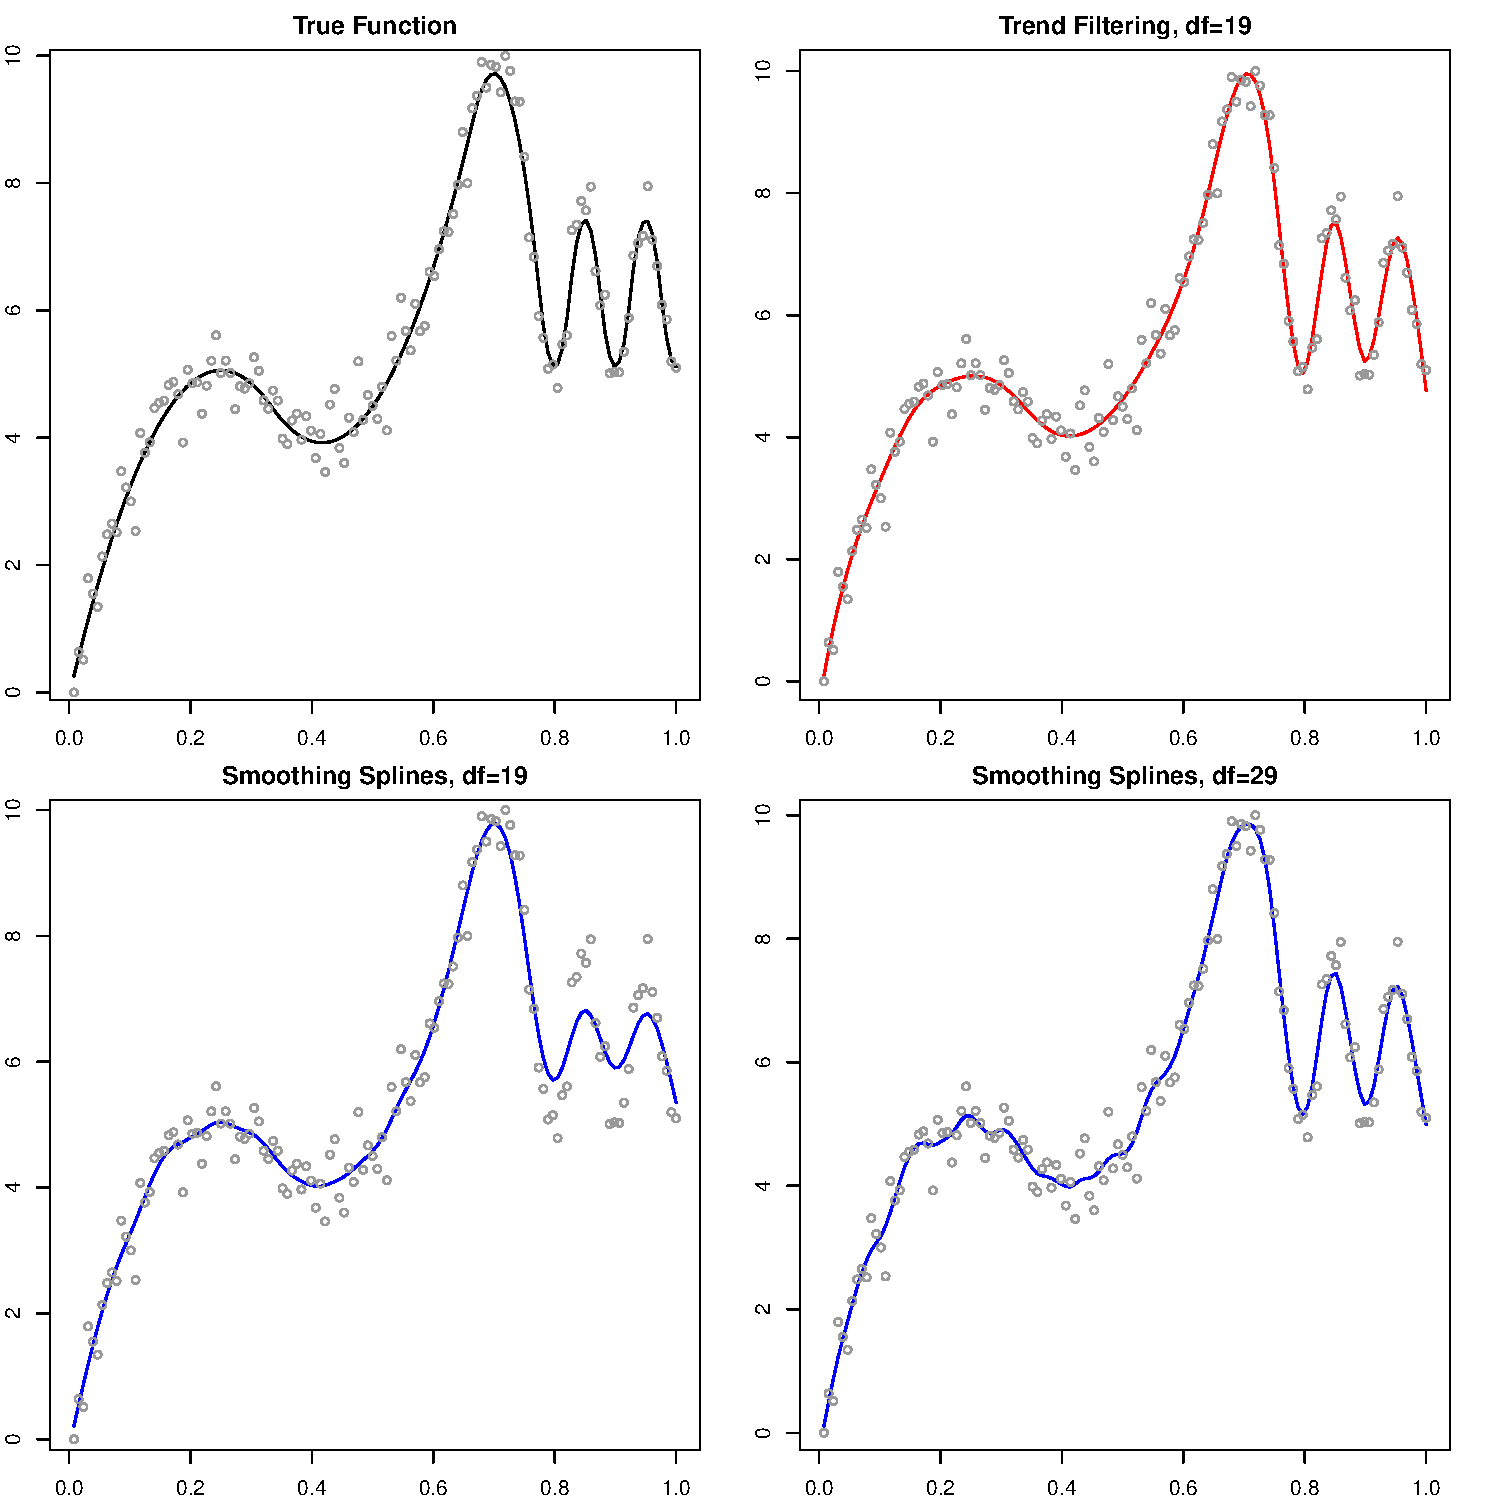
\includegraphics[width = 0.6\textwidth]{Figures/Figure4.pdf}
\caption{Comparison of trend filtering and smoothing spline over the same "hills" data consider in Figure \ref{fig:ssvslars}. The trend filtering fit with $df = 19$ shown in the top right panel clearly outperforms both smoothing spline fit.}
\label{fig:Figure4_ssvstfhills}
\end{figure}

We will compare trend filtering and smoothing spline of order $k = 3$. For cubic smoothing spline, the \textit{smooth.spline} function in R is extremely fast. To demonstrate trend filtering is more locally adaptive than smoothing spline, we will compare the performance of two methods over two simulation datasets: the "hills" data in the top left panel of Figure \ref{fig:ssvslars}, and the classical Doppler data. 


The fitted value of smoothing spline and trend filtering of order $3$ is shown in Figure \ref{fig:Figure4_ssvstfhills}. The defect of smoothing spline has been shown in the Introduction section. The fit of trend filtering with 19 degrees of freedom accurately captures the "hills" shape on the right end while successfully maintaining the smoothness on the left end. It adapts better to the heterogeneous "hills" than smoothing spline.

\begin{figure}[t]
\centering
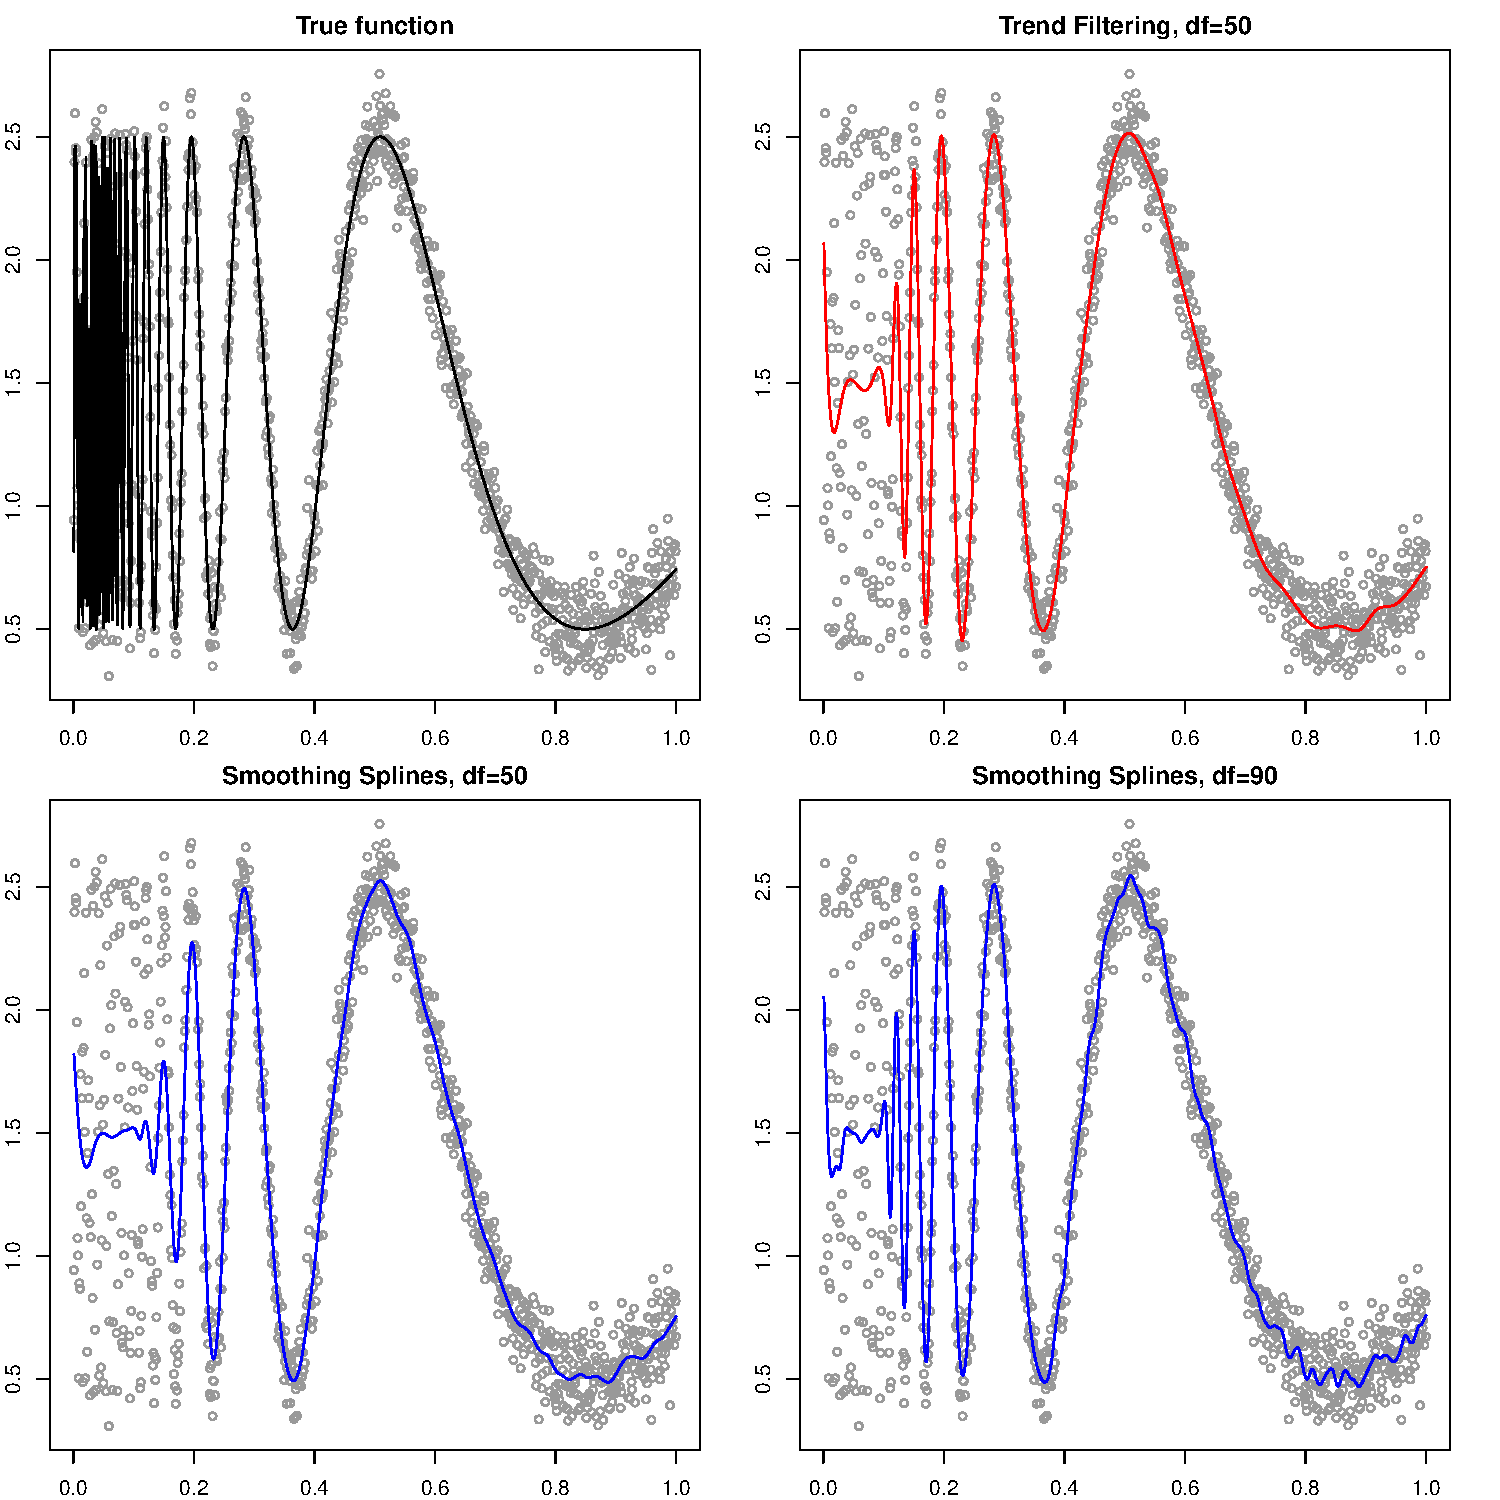
\includegraphics[width = 0.6\textwidth]{Figures/Figure5.pdf}
\caption{Comparison of trend filtering and smoothing spline over the heterogeneous Doppler data. Top left panel: true function with noisy observations; top right panel: trend filtering fit with 50 degrees freedom; bottom left panel: smoothing spline with 50 degrees of freedom; bottom right panel: smoothing spline with 90 degrees of freedom. Same defect of smoothing spline appear as in the "hills" data. Small degrees of freedom leads to over-smoothing of the oscillation on the left while large degrees leads to under-smoothing of the relatively smooth part on the right.}
\label{fig:Figure5_ssvstfdoppler}
\end{figure}

We then compare smoothing spline and trend filtering on another well-known heterogeneous function--- the Doppler function. The true function with noise observations is shown in the top left panel of Figure \ref{fig:Figure5_ssvstfdoppler}. The signal can be seen to be highly inhomogeneous in terms of smoothness. The left part of the functions exhibits high-frequency oscillations while the low-frequency part on the right is relatively smooth. In the top right panel is the fit of cubic trend filtering with 50 degrees of freedom, which picks up 4 cycles in the high-frequency area and remains sufficiently smooth in the low-frequency area. Smoothing spline with 50 and 90 degrees of freedom are shown in the bottom panels. With 50 degrees of freedom (same as trend filtering), smoothing spline only recovers 3 cycles in the high-frequency area. However, with 90 degrees of freedom and more complexity, smoothing spline finally recovers 4 cycles in the left but becomes extremely wiggly on the right. 

\begin{figure}[t]
\centering
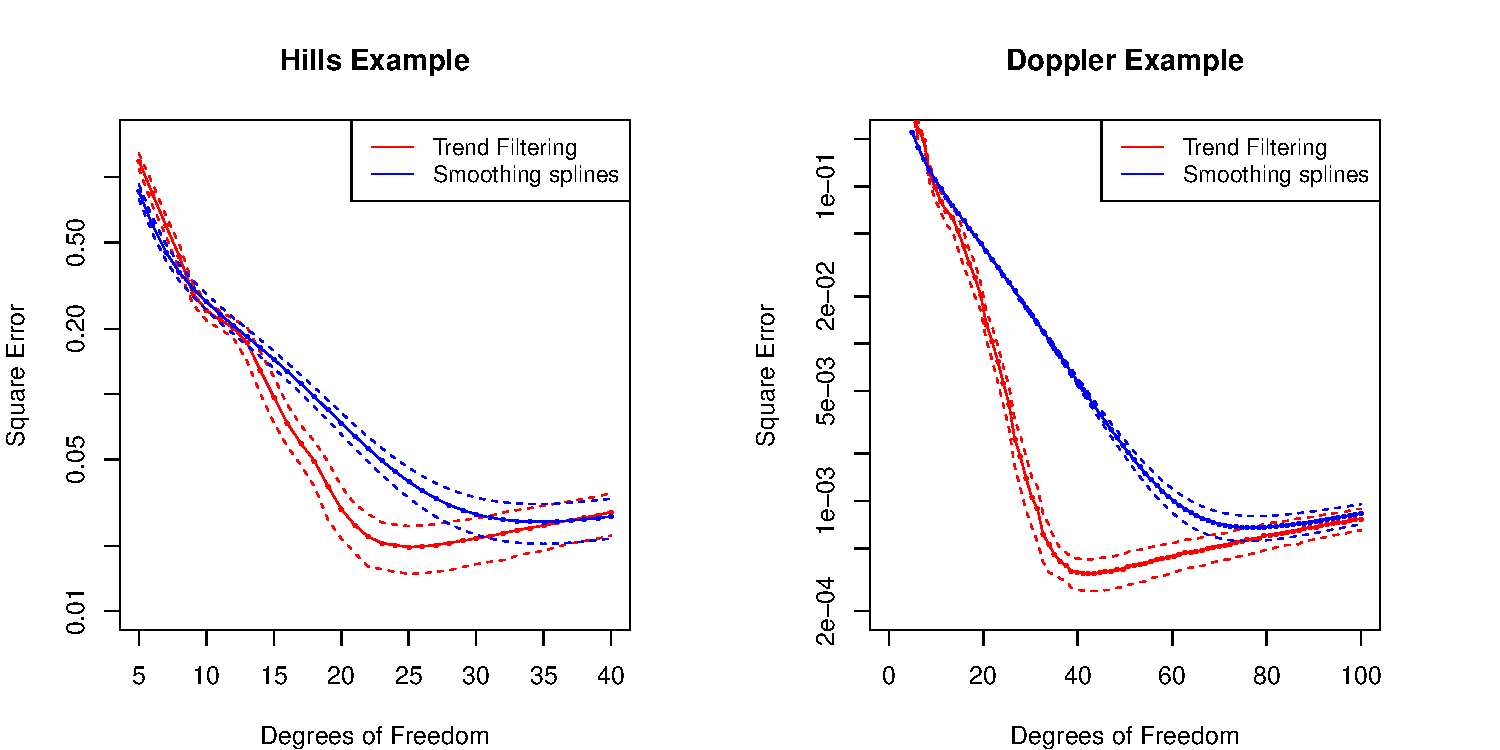
\includegraphics[width = 0.8\textwidth]{Figures/Figure6.pdf}
\caption{Comparison of cubic trend filtering and cubic smoothing spline in terms of MSE, for the "hills" data example on the left, and the Doppler example on the right. In each setup, trend filtering and smoothing spline estimators were fit over a range of degrees of freedom values. The red curves display the loss for trend filtering, and the blue curves for smoothing spline. The results were averaged over 50 simulated data sets, and the standard deviations are denoted by dotted lines. In these examples, trend filtering has a generally better predictive accuracy than smoothing splines, especially for models of low to intermediate degrees of freedom.}
\label{fig:Figure6_mse}
\end{figure}

Apart from visual comparison, we also quantitatively compare the performance of trend filtering and smoothing spline using mean square error(MSE). More specifically, we consider the following input-averaged squared error loss:
\begin{align}
\frac{1}{n}\sum_{i=1}^n (\hat{u}_i - f_0(x_i))^2 \quad \text{and}\quad \frac{1}{n}\sum_{i=1}^n (\hat{f}(x_i) - f_0(x_i))^2
\label{eq:avg_squareloss}
\end{align}
where $\hat{u}$ and $\hat{f}$ are the fit of trend filtering and smoothing spline respectively. We fit cubic trend filtering and cubic smoothing spline to the "hills" data and Doppler data using a wide range of model complexity indexed by the degrees of freedom. Figure \ref{fig:Figure6_mse} shows the MSE plot for the "hills" data and Doppler data respectively. We average the results over 50 simulated data sets and standard deviations are denoted by the dotted lines. It is easy to see that in terms of input-averaged square loss, trend filtering outperforms smoothing spline over a wide range of model complexity, especially for models of low to intermediate degrees of freedom. 

\subsection{Computational Comparison}
\label{subsec:sscomp}
Trend filtering has comparable computational cost with smoothing spline. Recall that smoothing spline can be recast into a ridge regression problem, as in \eqref{eq:ss_ridge} and in turn, we only need to solve the linear system as in \eqref{eq:ss_sol}. Depending on the basis $(\eta_1,\ldots, \eta_n)$ we choose, the computation of \eqref{eq:ss_sol} can be slow or fast. Specifically, if we choose the B-spline basis, the coefficient matrix $N^TN+\lambda\Omega$ has banded structure, thus the fit of smoothing spline for single $\lambda$ value can be solved in $\cal{O}(n)$ operations. In practice, these computations are extremely fast. 

For trend filtering, Algorithm I and Algorithm III introduced in Section \ref{subsec:algo} have computational cost $\cal{O}(n)$ and $\cal{O}(n^{3/2})$ respectively. In practice, the authors of \cite{kim2009ell_1} reported that the interior-point algorithm III has nearly $\cal{O}(n)$ cost. Thus trend filtering is computationally as efficient. Moreover, the path algorithm II solves the trend filtering problem for all $\lambda$ values with $\cal{O}(n)$ cost at each critical point of the solution path. Such path algorithm is especially useful when we consider a wide range of model complexity and fit trend filtering multiple times for different tuning parameter values.

\section{Comparison with Locally Adaptive Spline}
\label{sec:las_compare}

A more fair comparison for trend filtering is with another nonlinear smoother---locally adaptive spline. Locally adaptive spline was proposed in \cite{mammen1997locally} and, as its name suggests, has nice local adaptive properties. The original definition for locally adaptive spline in \cite{mammen1997locally} is via the following minimization problem:

\begin{align}
\hat{f} \in \argmin_{f\in\cal{F}_k} \frac{1}{2}\sum_{i=1}^n (y_i - f(x_i))^2 + \lambda\cdot\text{TV}(f^{(k)})
\label{eq:las_unconstrained}
\end{align}
where $\text{TV}(\cdot)$ is the total variation norm defined as 

\begin{align*}
\text{TV}(f) = \sup\{\sum_{i=1}^p |f(z_{i+1}) - f(z_i)|:z_1<z_2<\ldots<z_p \text{ is a partition of [0, 1]}\}
\end{align*}
and this is reduced to $\text{TV}(f) = \int_0^1|f'(t)|dt$ is $f$ is differentiable. The domain function class in \eqref{eq:las_unconstrained} is called the $k$th order bounded total variation class defined as 

\begin{align*}
\cal{F}_k = \{f:[0, 1]\rightarrow\RR: f \text{ is $k$ times weakly differentiable and TV($f^{(k)}$)$<\infty$}\}
\end{align*}
Note that $\cal{F}_k$ is a function space with infinite dimension, thus similar to smoothing spline, the original definition of locally adaptive spline is infinite-dimensional. Remarkably, \cite{mammen1997locally} proved that one of the solutions to \eqref{eq:las_unconstrained} is a $k$th order spline(the $\in$ sign in \eqref{eq:las_unconstrained} marks non-unique solutions). Define the knot superset

\begin{align}
T = 
\begin{cases}
\{x_{k/2+2}, \ldots, x_{n-k/2}\} & \text{if $k$ is even}\\
\{x_{(k+1)/2+1, \ldots, x_{n-(k+1)/2}}\} & \text{if $k$ is odd}
\end{cases}
\label{eq:knotT}
\end{align}
then \cite{mammen1997locally} proved that for $k = 0$ and $k = 1$, the minimum of \eqref{eq:las_unconstrained} can be achieved with a $k$th order spline with knots contained in $T$. However, this is not necessarily true for $k\geq 2$, as the solution spline can have knots outside the inputs $\{x_1,\ldots, x_n\}$. Thus we claim that locally adaptive spline is intrinsically hard to solve for order $k\geq 2$, and to make it more computationally tractable, we resort to its constrained form

\begin{align}
\hat{f} = \argmin_{f\in\cal{G}_k} \frac{1}{2}\sum_{k=1}^n (y_i - f(x_i))^2 + \lambda\cdot\text{TV}(f^{(k)})
\label{eq:las_constrained}
\end{align}
where $\cal{G}_k$ is the constrained function class
\begin{align*}
\cal{G}_k = \{f:[0, 1]\rightarrow\RR:\text{$f$ is $k$th order spline with knots contained in $T$}\}
\end{align*}
To summarize the discussion before, the solution to the constrained problem  \eqref{eq:las_constrained} is also solution to the unconstrained problem \eqref{eq:las_unconstrained} for $k = 0, 1$ but not for $k\geq 2$. Fortunately, \cite{mammen1997locally} shows that essentially all of their theoretical results for the unconstrained problem \eqref{eq:las_unconstrained} also apply to the constrained problem \eqref{eq:las_constrained} as long as the inputs $(x_1,\ldots, x_n)$ are not too far away. In particular, when the inputs are evenly spaced, i.e. $x_i=\frac{i}{n}$ for $i=1,\ldots, n$, the convergence rate of the solutions to the constrained problem and unconstrained problem are the same. For the rest of the paper, we will focus on the constrained form of locally adaptive spline. 

\subsection{Locally Adaptive Spline as Lasso Type Problem}
\label{subsec:lasaslasso}
We show in this subsection that the constrained locally adaptive spline problem can also be represented in (generalized) Lasso form. Note that the knot superset $T$ has $n-k-1$ elements, easy computations shows that the class of $k$th order spline with knots in $T$ has $n$ basis functions. Write the basis as $(g_1,\ldots, g_n)$ and $T = \{t_1,\ldots, t_{n-k-1}\}$ with extra definition $t_0 = 0$, then

\begin{align*}
\text{TV}(g_j^{(k)}) = \sum_{i=1}^{n-k-1} |g_j^{(k)}(t_i) - g_j^{(k)}(t_{i-1})|
\end{align*}
and any linear combination of the basis $\sum_{i=j}^n \theta_jg_j$ has total variation norm

\begin{align*}
\text{TV}((\sum_{j=1}^n\theta_jg_j)^{(k)}) = \sum_{i=1}^{n-k-1}|\sum_{j=1}^n (g_j^{(k)}(t_i) - g_j^{(k)}(t_{i-1}))\cdot\theta_j|
\end{align*}
Thus \eqref{eq:las_constrained} can be equivalently written as

\begin{align}
\hat{\theta} = \argmin_{\theta\in\RR^n} \frac{1}{2}\|y-G\theta\|_2^2 + \lambda\|C\theta\|_1
\label{eq:las_genlasso}
\end{align}
which is a generalized Lasso problem with design matrix $G$ and penalty matrix $C$. The solution to \eqref{eq:las_constrained} is recovered by $\hat{f} = \sum_{j=1}^n \hat{\theta}_jg_j$. Here $G$ is the evaluations of $(g_1,\ldots, g_n)$ over the inputs $(x_1,\ldots, x_n)$ and $C$ contains the difference of $k$th order derivatives of $(g_1,\ldots, g_n)$ at consecutive knots. In words,

\begin{equation}
\begin{aligned}
&G_{ij} = g_j(x_i) \quad i,j = 1,\ldots, n\\
&C_{ij} = g_j^{(k)}(t_i) - g_j^{(k)}(t_{i-1}) \quad i = 1,\ldots, n-k-1, j= 1,\ldots, n
\label{eq:lars_design}
\end{aligned}
\end{equation}

Note that \eqref{eq:las_genlasso} indicates that locally adaptive spline is a generalized Lasso problem. Depending on different choice of the basis functions $(g_1,\ldots, g_n)$, the design matrix $G$ and penalty matrix $C$ will have different structures. In particular, if we choose $(g_1,\ldots, g_n)$ as the truncated power basis defined in \eqref{eq:trun_basis}, \eqref{eq:las_genlasso} can be further transformed into an ordinary Lasso problem. 

\begin{lemma}
Let $T$ be the knot superset defined in \eqref{eq:knotT}, and $(g_1,\ldots, g_n)$ chosen as the truncated power basis defined in \eqref{eq:trun_basis}. Then the locally adaptive spline problem \eqref{eq:las_constrained} is equivalent to the following Lasso problem:
\begin{align}
\hat{\theta} = \argmin_{\theta\in\RR^n}\frac{1}{2}\|y-G\theta\|_2^2 + \lambda\sum_{j=k+2}^n |\theta_j|
\label{eq:las_lasso}
\end{align}
in that $\hat{f}(x) = \sum_{j=1}^n \hat{\theta}_jg_j(x)$ for $x\in[0, 1]$. Design $G$ is defined in \eqref{eq:lars_design}.
\label{lemma:las_lasso}
\end{lemma}

The proof of the Lemma \ref{lemma:las_lasso} is easy. We just plug the truncated power basis \eqref{eq:trun_basis} into \eqref{eq:lars_design} and obtain a more succinct representation of the penalty matrix $C$. However, Lemma \eqref{lemma:las_lasso} is very useful because it enables us to directly compare locally adaptive spline and trend filtering by noticing that trend filtering also has an equivalent Lasso form \eqref{eq:tf_lasso}. Notice that \eqref{eq:las_lasso} and \eqref{eq:tf_lasso} have exactly the same Lasso form except for the design matrix. Now if we compare the two design matrices $G$ and $H$, it is not hard to see that for $k = 0$ and $k = 1$, $G = H$, thus the fits of trend filtering and locally adaptive spline are exactly the same. For $k\geq 2$, however, $G$ is generically not the same as $H$, thus the fits of the two methods will differ. The next lemma formalize this result. 

\begin{lemma}
Consider evenly-spaced inputs $x_i = \frac{i}{n}$ for $i= 1,\ldots, n$, and the design matrix $H$ and $G$ defined in \eqref{eq:tf_lasso} and \eqref{eq:las_lasso}. For $k = 0, 1$, the solutions to locally adaptive spline and trend filtering with the same tuning parameter $\lambda$ are the same, i.e.

\begin{align*}
\hat{u}_i = \hat{f}(x_i) \quad i=1,\ldots, n
\end{align*}
where $\hat{u}$ and $\hat{f}$ are the solutions to trend filtering and locally adaptive spline respectively.

For $k\geq 2$, $G\neq H$, thus the solutions to the two methods will be generically different. 
\label{lemma:lasequivtf}
\end{lemma}

Even though Lemma \eqref{lemma:lasequivtf} shows that the solutions of trend filtering and locally adaptive spline of order $k\geq 2$ are generally different, we will show in the next subsection that in practice, these two methods have very similar fits. 

\subsection{Empirical Comparison}
\label{subsec:emplasvstf}

\begin{figure}[t!]
\centering
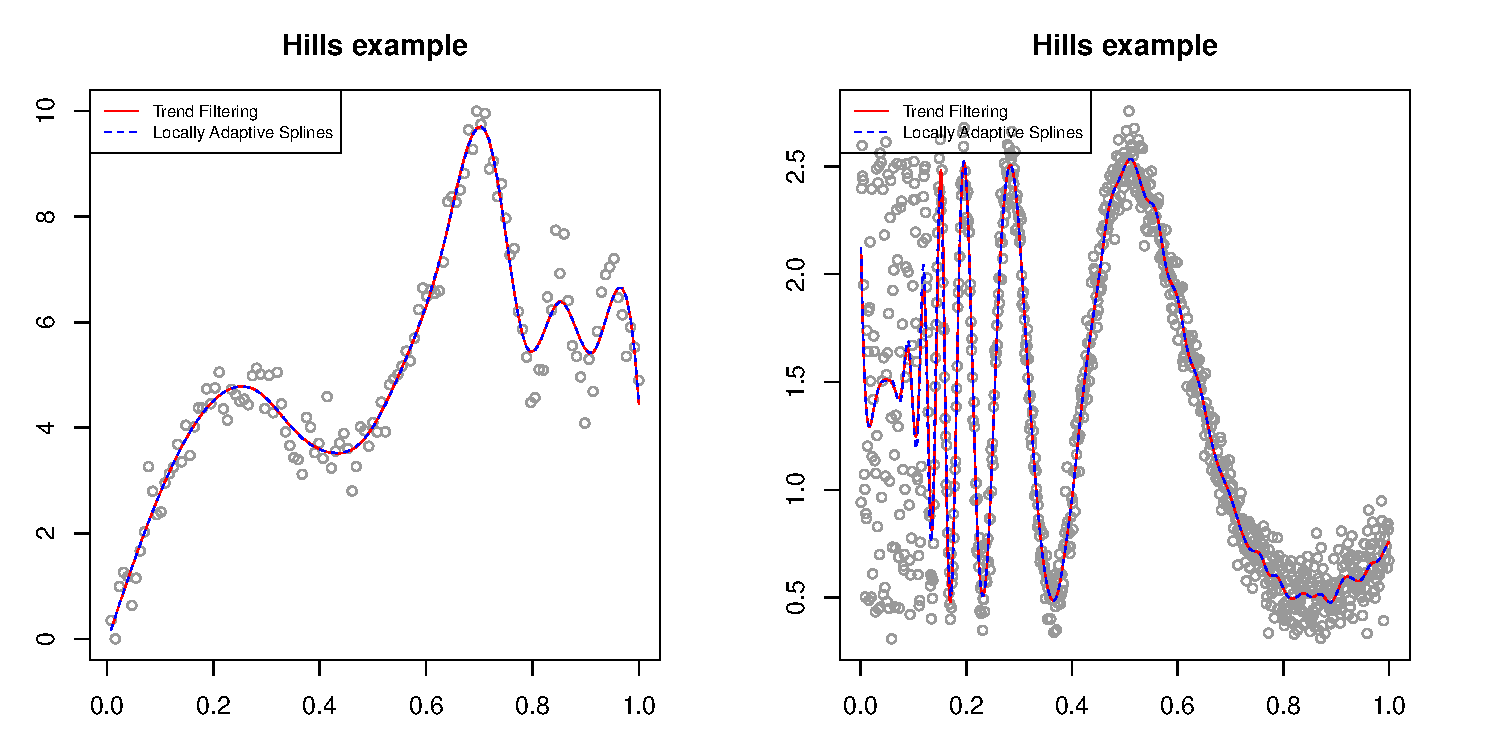
\includegraphics[width = 0.8\textwidth]{Figures/Figure7.pdf}
\caption{Comparison of cubic trend filtering and locally adaptive spline ($k = 3$) with the same tuning parameter on the "hills" data and Doppler data. Left panel shows the "hills" data, and the right panel shows the Doppler data. The fits of the two methods can be seen to be extremely similar. Except for some tiny difference at $x= 0.1$ in the Doppler data, the difference between these two methods are only numerical.}
\label{fig:Figure7_lasvstf}
\end{figure}

In this subsection we empirically compare the fits of trend filtering with locally adaptive spline. We will revisit the two heterogeneous signals considered in Section \eqref{subsec:sssimu}. Figure \ref{fig:Figure7_lasvstf} compares these two methods on the "hills" data and Doppler data. Fits of the two methods can be seen to be extremely similar. There is no visible difference for the "hills" data, and very tiny difference at $x = 0.1$ in the Doppler data. Even though we only show here the case for $k = 3$, such similarity exists for all orders in our simulation. We will prove in the next section that asymptotically, the fits of these two methods with the same tuning parameter converge to each other. However, their similarity in finite samples is beyond the explanation in this paper and is still an open question.

\subsection{Computational Comparison}
One way to solve the locally adaptive spline is to solve its Lasso form \eqref{eq:las_lasso} or its generalized Lasso form \eqref{eq:las_genlasso}. To make computation efficient, we need to choose an appropriate basis $(g_1,\ldots,g_n)$ so that the penalty matrix $C$ and design matrix $G$ are as sparse as possible. There is a dilemma here though. One the one hand, the truncated power basis \eqref{eq:trun_basis} will make penalty $C$ identity but design $G$ dense. On the other hand, to make the design $G$ sparse, we need to choose basis with local support, for example, the B-spline basis, which, however, will make the penalty $C$ dense. Therefore we are more of less stuck with a dense (generalized) Lasso problem.

Authors of \cite{mammen1997locally} proposes an alternative to solve the locally adaptive spline. For $k = 1$, the proposed algorithm solves \eqref{eq:las_constrained} for a given $\lambda$ in $\cal{O}(n\log(n))$ operations and $\cal{O}(n^2)$ operations for all $\lambda$. However, there is no guaranteed cost of the algorithm for higher orders ($k\geq 2$)(the authors conjecture the algorithm takes also $\cal{O}(n^2)$ operations for all $\lambda$). We therefore conclude that locally adaptive spline is not as computationally efficient as trend filtering. 

\section{Real Data Study}
\label{sec:real_data}

\begin{figure}[t!]
\centering
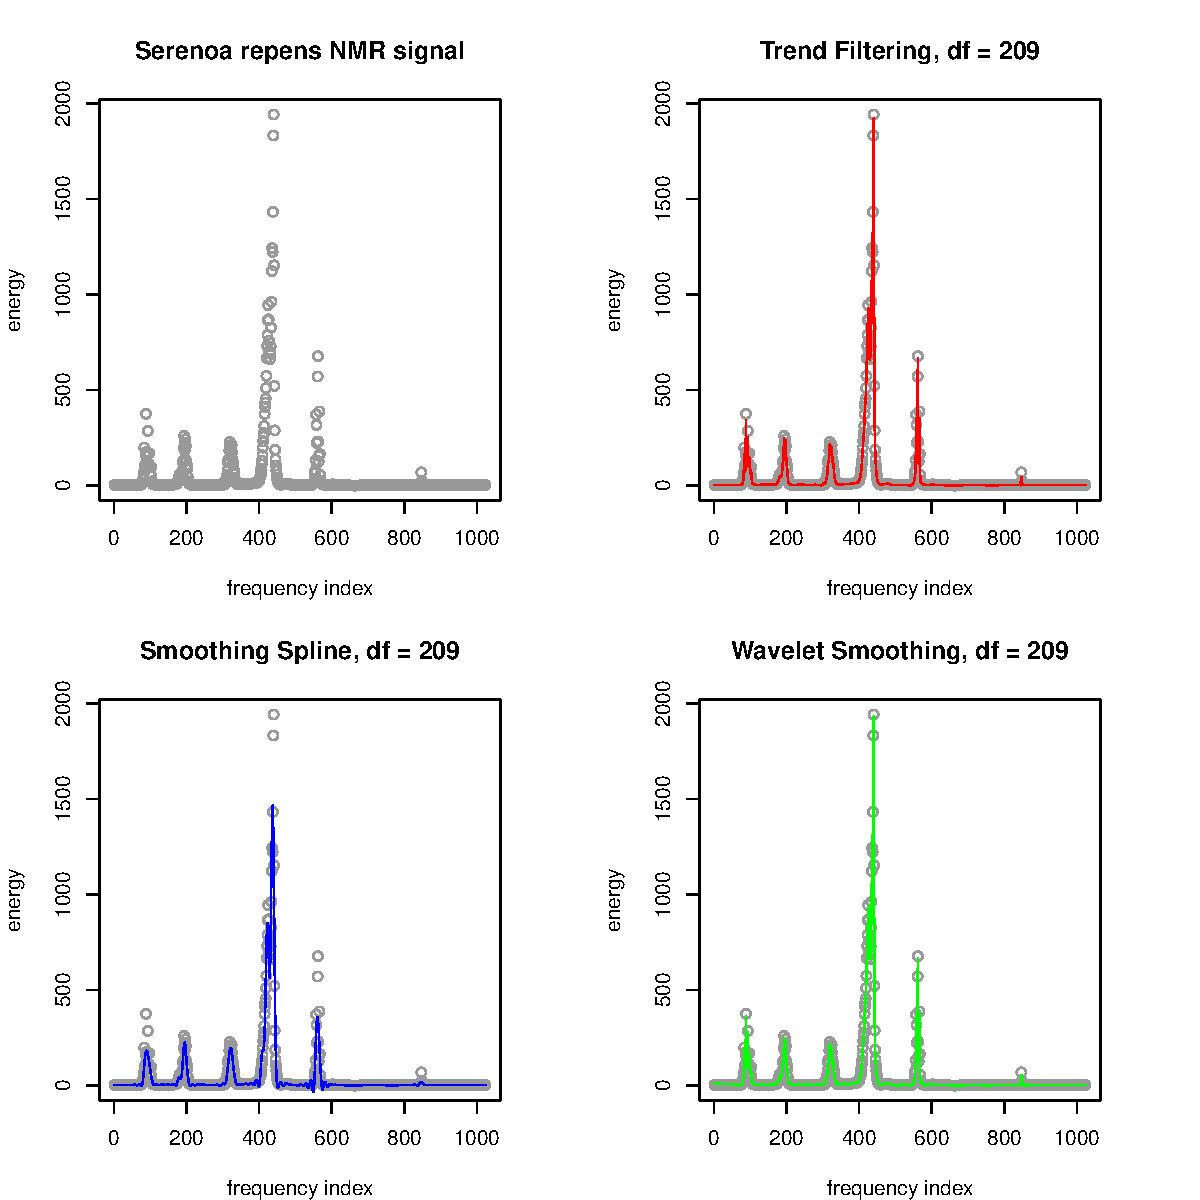
\includegraphics[width = 0.9\textwidth]{Figures/Figure9.pdf}
\caption{The top left panel shows $n=1024$ measurements of frequency and energy in a NMR spectrum. The top right panel shows the fit of cubic trend filtering with 209 degrees of freedom(which is chosen through cross-validation). The bottom left panel and bottom right panel show the fit of smoothing spline and wavelet with the same degrees of freedom. Smoothing spline clearly over-smoothes the spikes(especially the 1st, 4th and 5th one). Trend filtering and wavelet smoothing give very similar fit and both perform very well on both the smooth part and the spikes. Close inspection shows that trend filtering does slightly better at the smooth part, as wavelet estimate is slightly wiggly at the transitions between flats and spikes.}
\label{fig:Figure_9}
\end{figure}


In this section, we examine one of the Nuclear Magnetic Resonance (NMR) spectra data to compare the performance of different methods. The data is available at \url{https://github.com/bryanhanson/ChemoSpec}. This data contains a collection of 14 NMR spectra of essential oil extracted from the
palm \emph{Serenoa repens} or Saw Palmetto, which is commonly used to treat
benign prostatic hyperplasia (BPH) in men. The NMR uses the magnetic properties of atomic nuclei to get information about an oil sample. The $x$ axis indexes the frequency of the spectrum, which in our oil sample there are 32,768 frequencies. The $y$ axis marks the corresponding amount of energy in that frequency. Since a large part of the frequencies have close to 0 energy, we choose an informative segment of $n = 1024$ frequencies and corresponding energy count. The true measurement is shown in the top left panel of Figure \ref{fig:Figure_9}.

We compare the performance of trend filtering, smoothing spline and wavelet smoothing. The fit of locally adaptive spline is omitted here due to its extreme similarity to trend filtering, as shown in Section \ref{sec:las_compare}. The smoothing spline is implemented by the \textit{smooth.spline} function in R, and wavelet smoothing is implemented by the \textit{wavethresh} package in R. The "wavelets on the interval" option in the \textit{wd} function in the \textit{wavethresh} package is chosen to handle the boundary conditions (as periodicity and symmetry are not appropriate assumptions for the boundary behavior in this example), which uses the algorithm of Cohen, Daubechies and Vial\cite{cohen1993wavelets}. Note that wavelet smoothing usually requires the sample size $n$ to be a power of $2$, thus we choose our segment length as $1024$ to accommodate this requirement. We use the continuous time representation from Section \ref{subsec:ct_tf} and cross validation to choose the best degrees of freedom for trend filtering, which gives us $df = 209$, we then calibrate the fit of smoothing spline and wavelet using this same degrees of freedom.

The estimates of trend filtering, smoothing spline and wavelet smoothing are shown in the top right panel, bottom left panel and bottom right panel of Figure \ref{fig:Figure_9} respectively. Trend filtering clearly outperforms smoothing spline in this case as smoothing spline severely over-smoothes the spikes, especially the 1st, 4th and 5th one. Wavelet smoothing gives very similar estimate to trend filtering, performing pretty well on both the smooth part and the spikes. Close inspection shows that trend filtering does slightly better at the smooth part, as the wavelet estimate is slightly wiggly at the transitions between flats and spikes.

\bibliography{paperreview}
\end{document}